\subsection{Calibration of the VMM ASIC}
\label{sec:calib_alg}

\begin{figure}[!htb]
    \begin{center}
        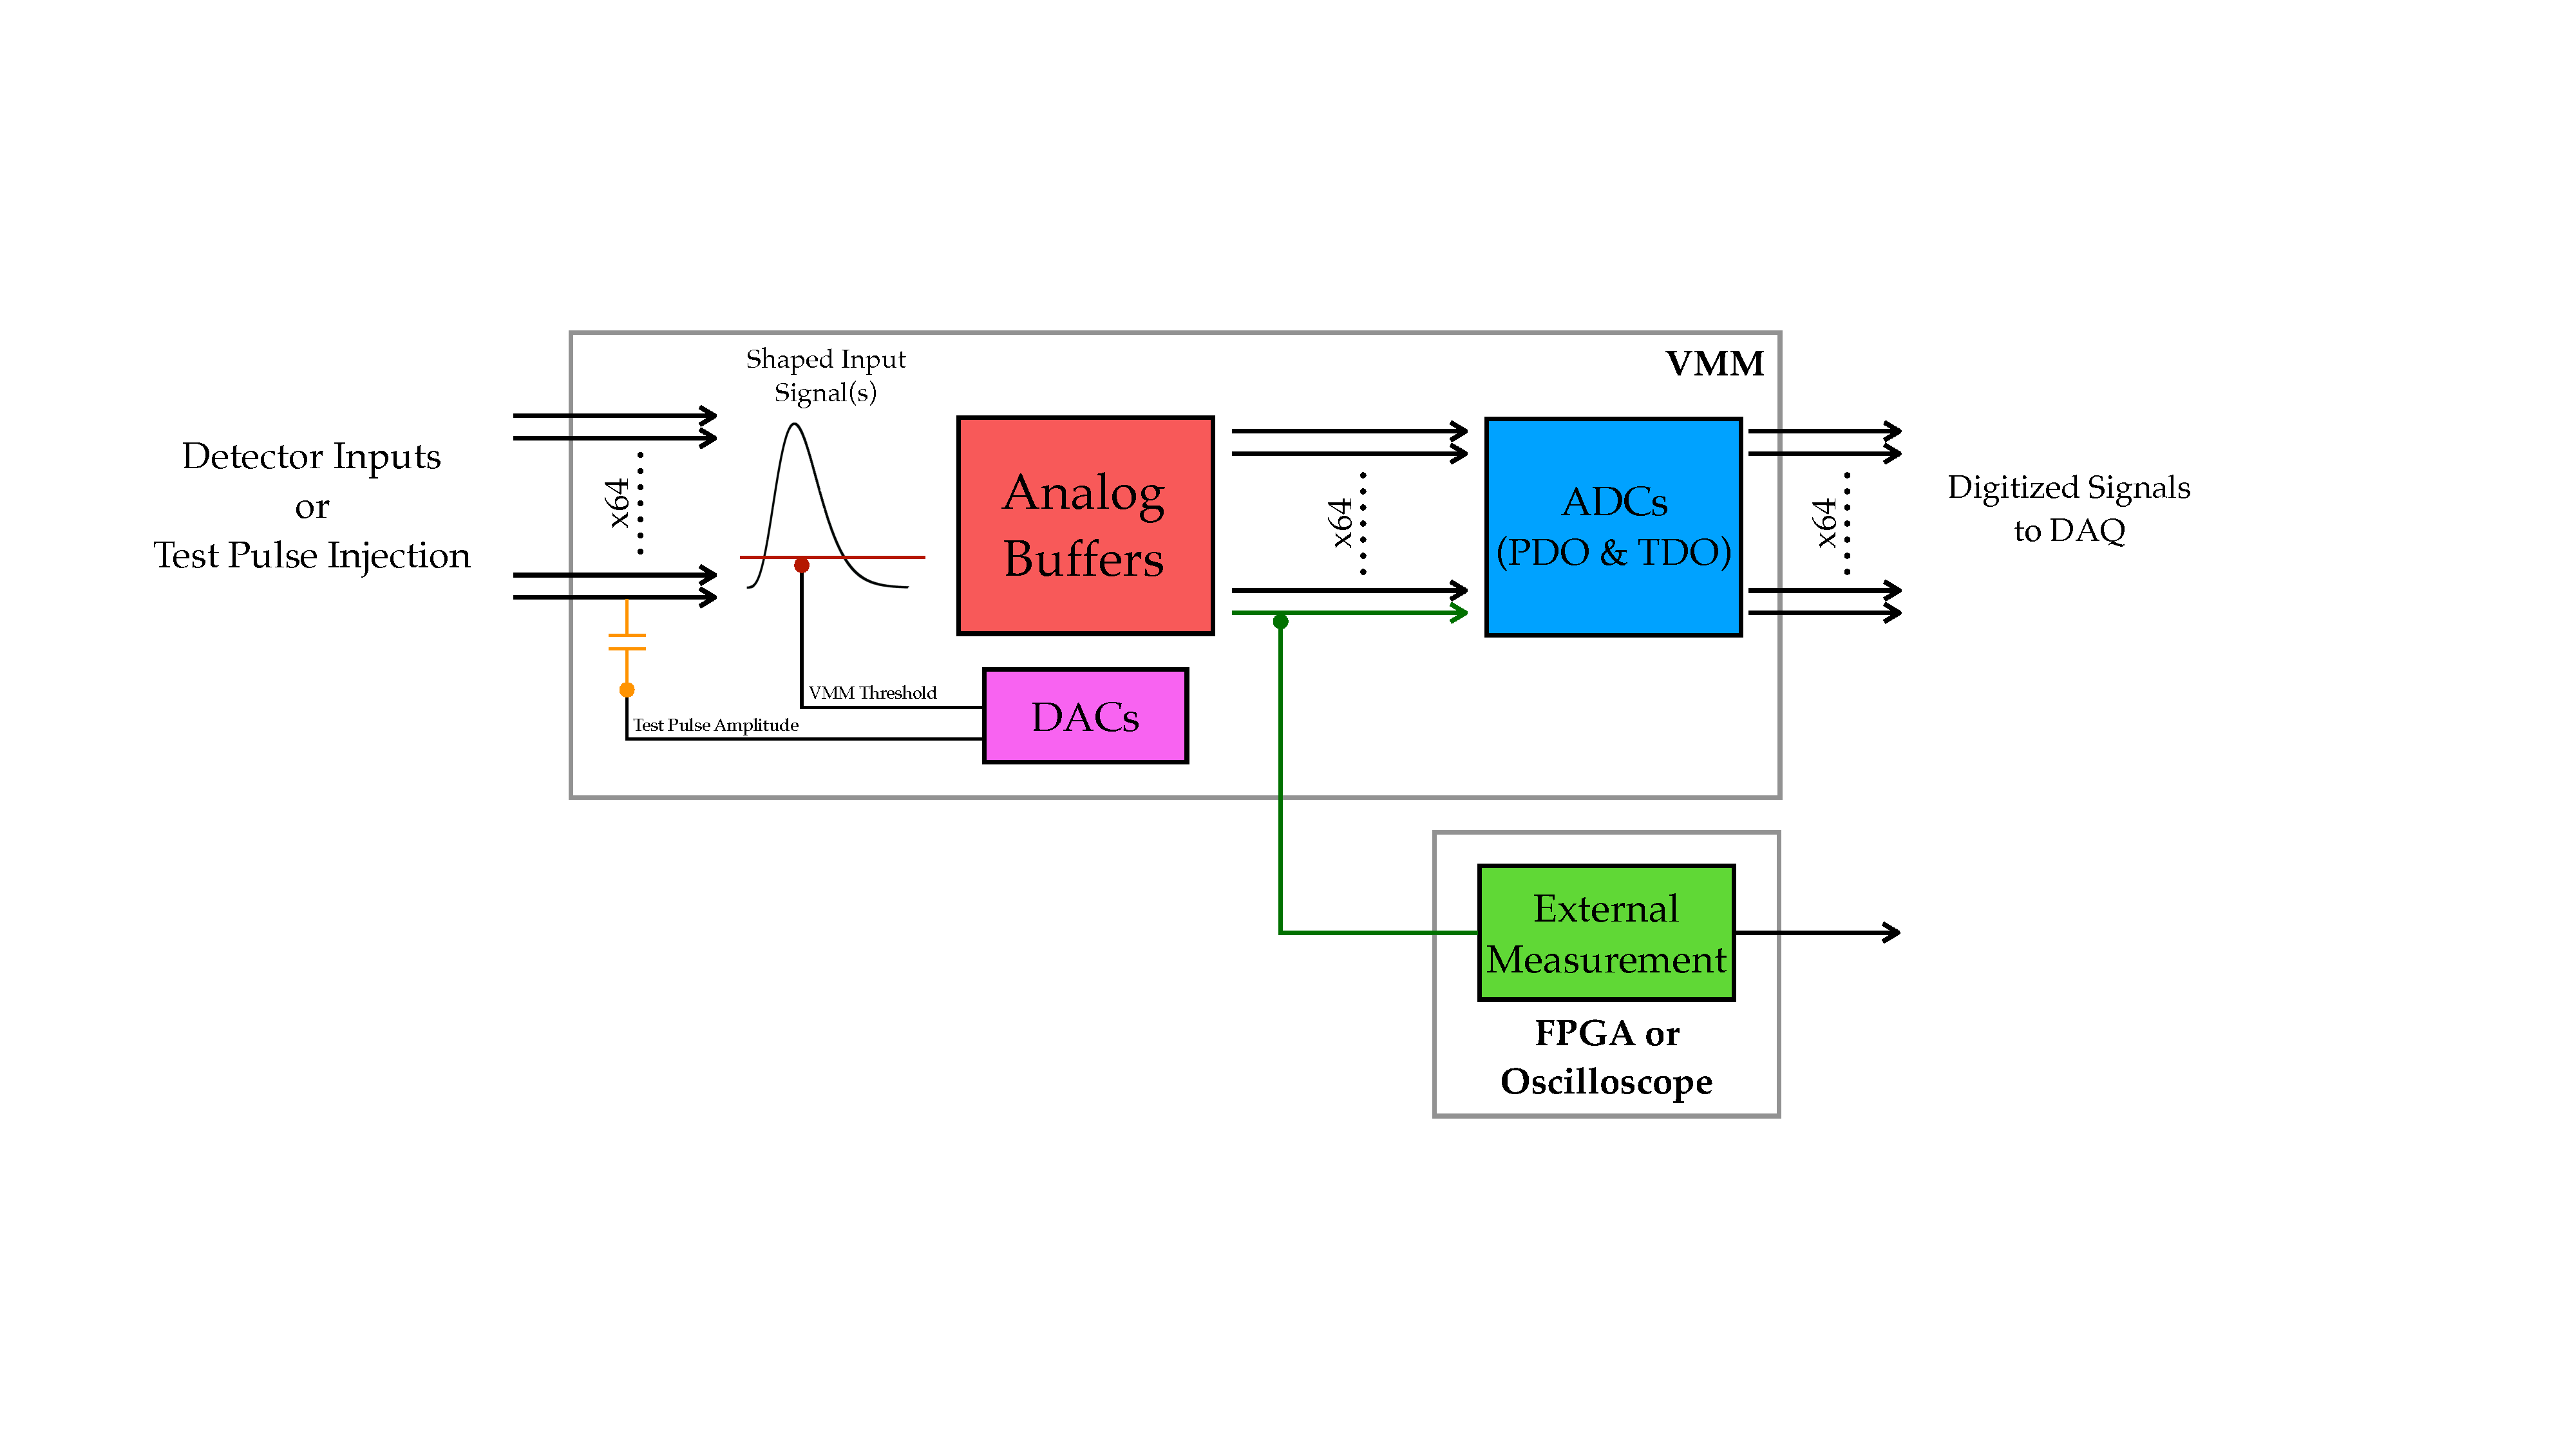
\includegraphics[width=0.8\textwidth]{figures/nsw/calibration/xadc_diagramPDF}
        \caption{
            Illustration of the concept of using an external measurement for calibration
            of the VMM internals.
            For the automated calibration routines described in the text, the ADC provided
            by the FPGA is used as the external measurement device but an oscilloscope probe can be used
            as well.
            For calibration purposes, the external measurements are of the VMM channel analog outputs prior
            to digitisation via the internal VMM ADCs
            (green), the VMM threshold DAC analog output (red circle), and the
            output of the DAC setting the test pulse amplitude (yellow) provided by the test charge capacitor
            on each VMM channel.
            Not indicated, external measurements are also made of each of the VMM channel's discriminator thresholds.
        }
        \label{fig:xadc_diagram}
    \end{center}
\end{figure}

As mentioned above, the VERSO software performs automated calibrations of
the frontend electronics.
The types of signals being collected on the NSW detectors are characterised by
very low signal amplitudes and are therefore typically noise dominated, with
much of the noise component derived mainly from the frontend electronics themselves.
It is therefore necessary to optimise the readout functionality of the
the VMM ASIC by calibrating it and ensuring that its signal-to-noise
ratio, $S/N$, is maximised during data taking.
Additionally, to achieve the best performance in the reconstruction of particle
tracks in the NSW detectors, several key aspects such as the charge amplitude
and timing measurement of the VMM need to be understood and well calibrated.
In this section a few of the calibration routines supported by VERSO will be discussed.

Many of the VMM calibrations rely on an external measurement of certain VMM characteristics
to be made.
These measurements are made using absolute measurements independent of any of the
internal VMM measurement mechanisms.
The VMM has built-in multiplexing capabilities that allow for it to route analog signals
to the MO output described in previous sections.
Specific for calibration, the VMM can route to MO any of the following:
\begin{description}
    \item[] \textbf{Channel Analog Output}: Analog levels of each channel's analog level prior to digitisation via the internal ADCs
    \item[] \textbf{Threshold DAC}: Analog output of the DAC controlling the global VMM threshold
    \item[] \textbf{Test Pulse DAC}: Analog output of the DAC controlling the test pulse amplitude
    \item[] \textbf{Channel Threshold Trimmers}: Analog measurement of each channel's discriminator's threshold voltage
\end{description}
On the frontend boards housing an FPGA, as in Figure~\ref{fig:frontend_boards}, the external measurement
is made by routing the MO output of a VMM to the built-in 12-bit ADC of the \textsc{Xilinx} FPGA, referred to as
the xADC.
The xADC has a full scale range of 1\,V, providing a digital measurement resolution of roughly 0.24\,mV.
The digitised samples produced by the analog measurements of the xADC are forwarded to the VERSO
DAQ software so that they can be stored and subsequently processed by the calibration algorithms.
As the xADC is housed in the on-board FPGA, the VERSO software can control its operation and access its measurements
using similar configuration and DAQ functionalities as described in the previous section.
Alternatively, the external measurement of the MO can be made via an oscilloscope probe.
The use of the oscilloscope probe does not lend itself to automated calibration but provides for
direct inspection of the analog levels as well as a reference on the measurements of the xADC.
An illustration of these external measurement mechanisms is provided in Figure~\ref{fig:xadc_diagram}.

\subsubsection{DAC Calibration}
\label{sec:calib_dac}

Each VMM has two important DACs: one for setting the global VMM threshold and one for
setting the amplitude of the injected test-pulse charge via the test-pulse capacitor on each
channel.
Each is 10-bit, meaning that it can be set to integer values between 0-1023 (inclusive).
In order for the user to know in absolute terms what the VMM threshold or test-pulse amplitude
is set to, i.e. in terms of analog voltage values and not digital counts, the analog level of each
DAC is measured using the xADC.
At each configured DAC value, between 0 and 1023, analog measurements are made of the DAC output and
the relationship between the output analog value and configured digital value can be obtained.
This is illustrated in Figure~\ref{fig:threshold_dac_calib} for a single VMM's threshold DAC.
A linear relationship is assumed and from a linear fit the \textit{DAC-mV} relation, giving
the mapping from the configured digital DAC value to its analog value observed by the VMM channels, is obtained
from the slope of the line.
The DAC-mV relation between VMMs is not necessarily the same, and therefore must be measured
for every single VMM in the system in order to be able to configure them all with the
same \textit{absolute} threshold or to inject test pulses with common amplitudes across VMMs.
Given the known capacitance of the test-pulse injection capacitor of the VMM channels,
the value of the injected charge for a configured test-pulse amplitude can be obtained via the $Q = C \cdot V$
relation, where $C$ is the injection capacitor's capacitance and $V$ is the test-pulse DAC output amplitude.%\footnote{
%The quoted capacitance value of the VMM channel's test-pulse injection capacitor, 3\,pF, is that of the
%VMM3 series of VMM. Earlier versions had lower capacitances.
%}

\begin{figure}[!htb]
    \begin{center}
        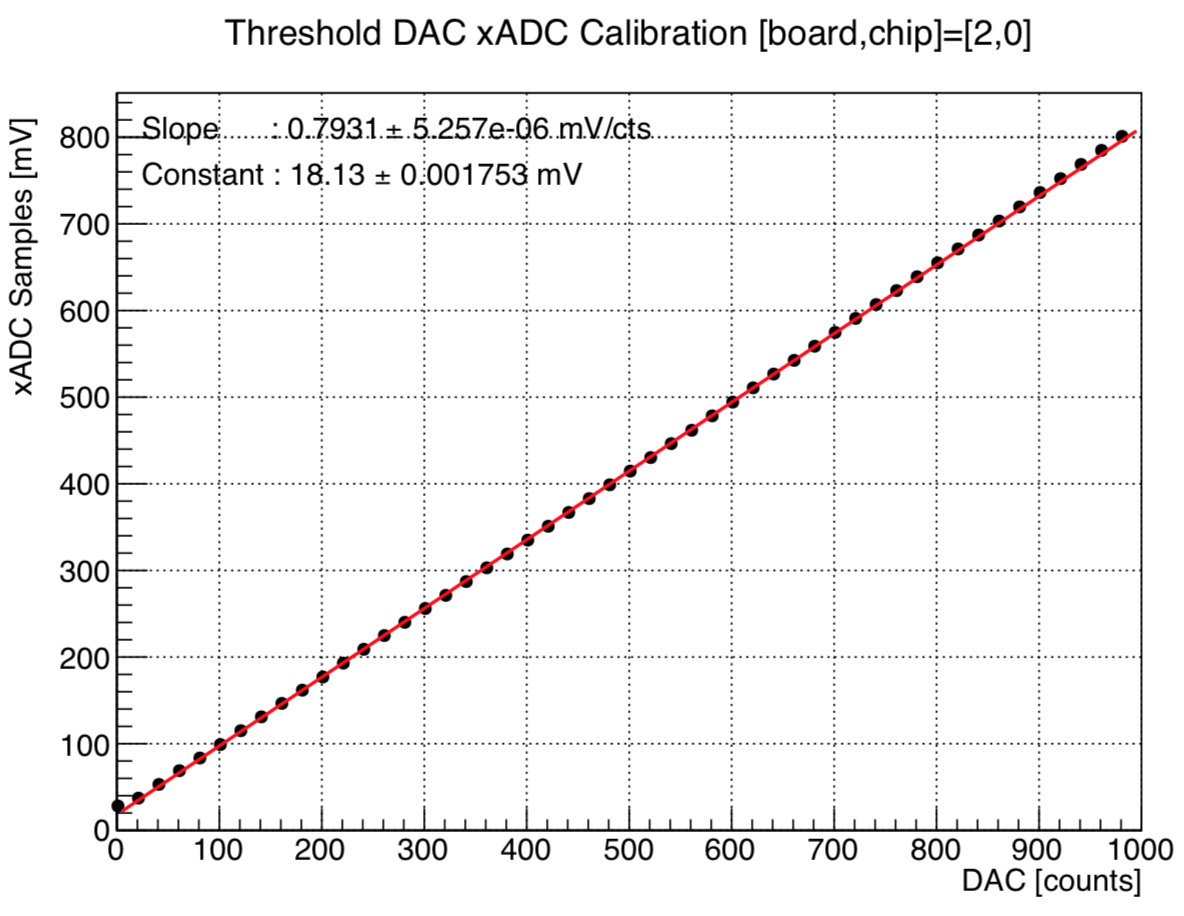
\includegraphics[width=0.6\textwidth]{figures/nsw/calibration/threshold_dac_calib}
        \caption{
            VMM global threshold measurement, using measurements made by the xADC, as a function
            of the set digital DAC value.
            The slope and y-intercept (`Constant') of the linear fit are provided.
            The slope gives the DAC-mV relation that allows for converting the digtal DAC
            configured value to an analog level at the VMM inputs.
        }
        \label{fig:threshold_dac_calib}
    \end{center}
\end{figure}

\subsubsection{Measurement of Channel Baselines and Noise}
\label{sec:calib_baselines}


External measurements via the xADC can be made of each channel's analog output (i.e. prior
to digitisation) when no signals are present at the channel input.
Doing so allows one to obtain a measurement of the channel \textit{baseline}, i.e. the
ambient level when no signal is present.
Fluctuations about the baseline, then, give a measurement of the inherent channel \textit{noise}.
Measurements of both of these quantities are important, both when the frontend electronics
are and are not interfaced to a detector.
Measurements of the noise when the frontend electronics are not interfaced to a detector give
a measurement of the inherent electronics noise characteristic of the frontend board.
Interfacing the frontend electronics to a detector introduces additional capacitive effects
that can introduce new sources of noise that must also be studied and perhaps reduced.
Knowledge of both the absolute baseline and noise levels of each VMM allows for the optimal threshold
to be set for the VMMs.
In order to be sensitive to small-amplitude signals, one would set the threshold just above the baseline
since the baseline defines the effective zero-level of an observable signal.
In practice, one sets the VMM threshold a few times the magnitude of the measured noise above the baseline: typically
2 to 3 times the level of the measured noise above the baseline.
Figure~\ref{fig:baselines_calib} shows an example of the measurements of a VMM channel's baseline and noise, taken by the xADC.
The xADC samples each channel's baseline and from the width of the distribution of these measurements the noise
level can be obtained.
Figure~\ref{fig:vmm_noise_enc} shows the evolution of the measured noise as a function of the VMM's
configured gain, both when the frontend board housing the VMM ASIC is and is not interfaced to a small prototype
MM detector having $\sim$30\,pF capacitance.

\begin{figure}[!htb]
    \begin{center}
        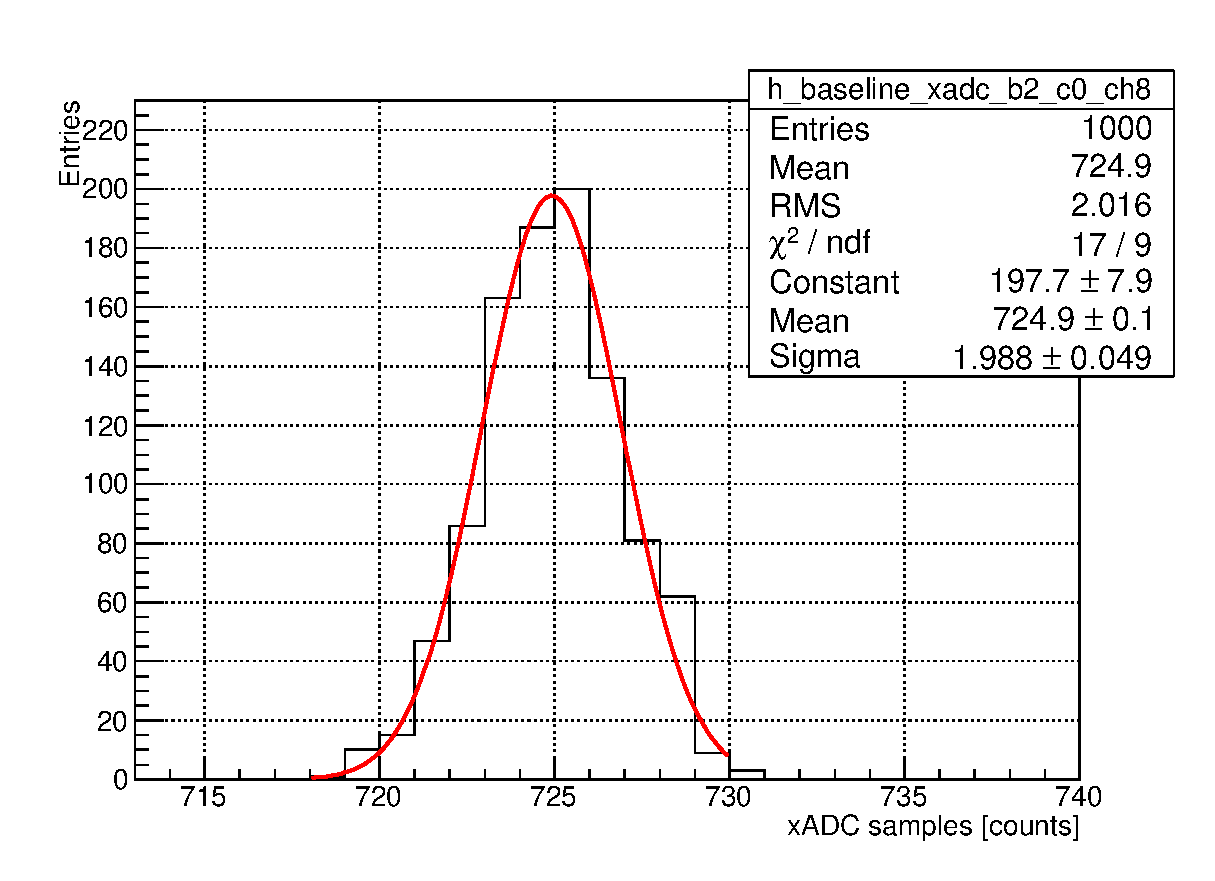
\includegraphics[width=0.46\textwidth]{figures/nsw/calibration/xadc_calib_channel_baseline_samples}
        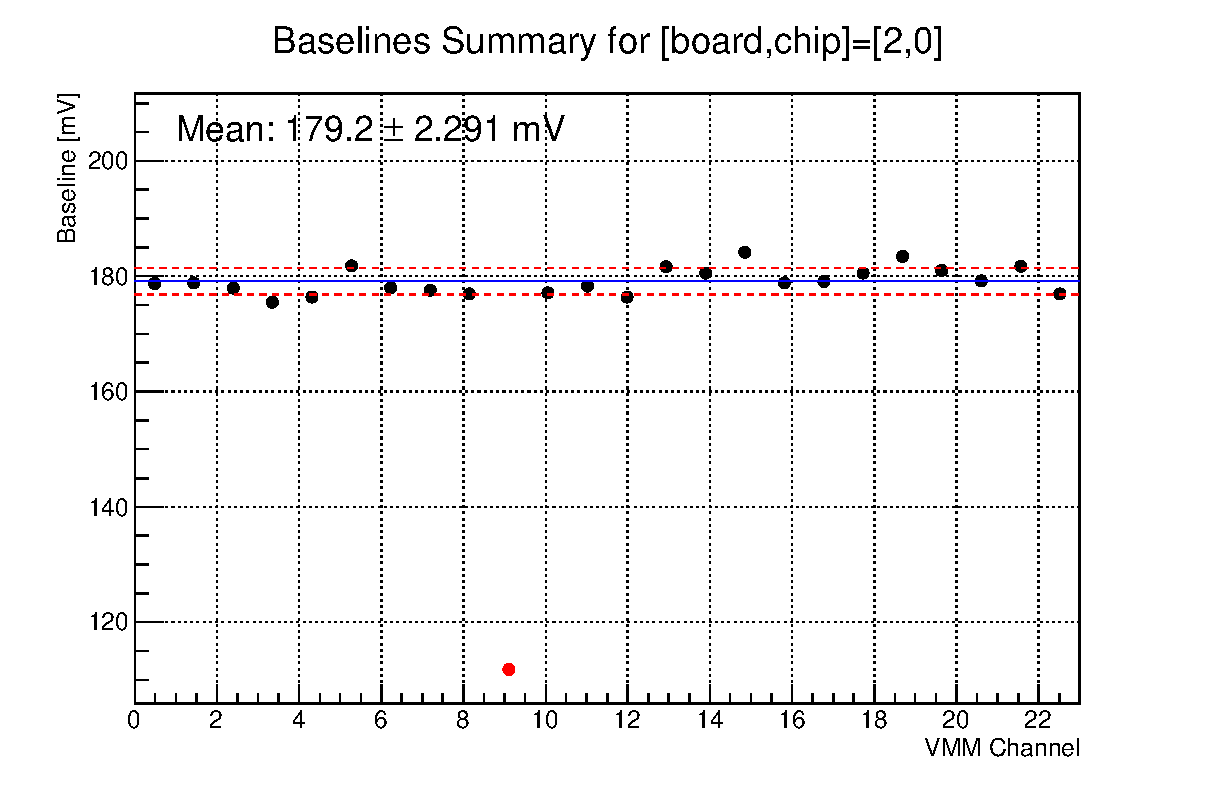
\includegraphics[width=0.53\textwidth]{figures/nsw/calibration/calib_baselines_vmm_summary}
        \caption{
            \textbf{\textit{Left}}: 1000 xADC measurements of a single VMM channel's input baseline.
                The width of the gaussian fit (red) gives the channel's noise level.
            \textbf{\textit{Right}}: Summary of the baseline measurements for 24 channels of a VMM.
                The error on the reported mean baseline, which is indicated by the blue line, is given by the RMS spread of the baseline measurements
                across all channels and is indicated by the red dashed lines.
                The channel with the red point (channel 9) is a faulty (dead) channel.
        }
        \label{fig:baselines_calib}
    \end{center}
\end{figure}

\begin{figure}[!htb]
    \begin{center}
        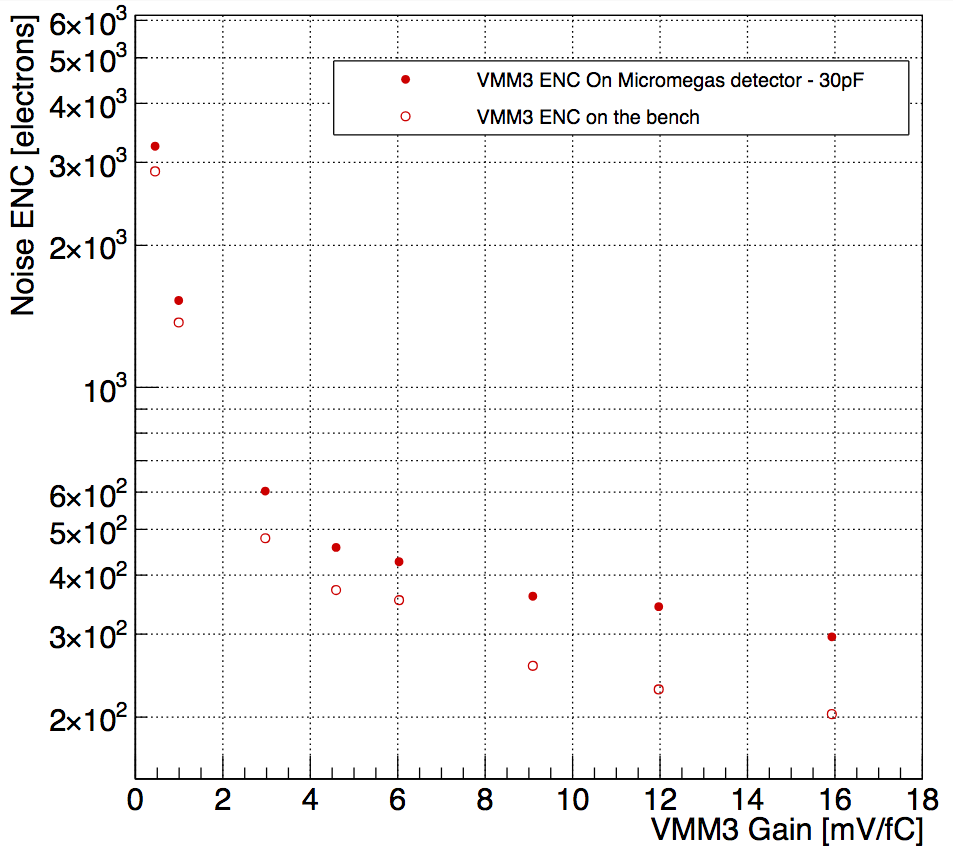
\includegraphics[width=0.5\textwidth]{figures/nsw/calibration/vmm_noise_enc}
        \caption{
            Equivalent noise charge (ENC) of the VMM3 as a function of its configured gain value.
            Noise measurements are performed with a GPVMM-type frontend board both on- (filled circles)
            and off-detector (unfilled circles).
            The detector used is a small $10\times10$\,cm$^2$ prototype MM chamber.
        }
        \label{fig:vmm_noise_enc}
    \end{center}
\end{figure}

\subsubsection{Channel Threshold Trimming}
\label{sec:calib_trimming}

The global VMM threshold inherently has channel-to-channel variation.
In order to ensure that the discriminators of all VMM channels in the system
fire at the same value, the VMM has a per-channel threshold trimming functionality included.
This functionality allows for each channel's threshold to be adjusted (`trimmed') in 32 steps that cover a range
of approximately 32\,mV.
To equalize the channel discriminators, external measurements made via the xADC are performed.
For each channel, measurements of the channel discriminator's threshold are taken at each of the 32
steps in the allowed range of trimming.
Once done for every VMM channel in the system, a metric for equalizing their thresholds is needed.
In the example of Figure~\ref{fig:calib_channel_trim}, the metric is to bring all channels
as close as possible to the globally set VMM threshold.
Once this is done, all VMM channels in the system ideally have equal thresholds and will
have equivalent responses to input signals.
As seen in Figure~\ref{fig:calib_channel_trim}, prior to this calibration there is quite
some variation, which shows the importance of this fine-grained calibration procedure.
The amount of threshold trimming necessary to bring a channel to its equalized state
is independent of the globally set VMM threshold; therefore, once the calibration procedure
is performed and the subsequent channel threshold trimming is applied, the global
threshold can be adjusted with confidence that all channels in the system are likewise adjusted coherently.

\begin{figure}[!htb]
    \begin{center}
        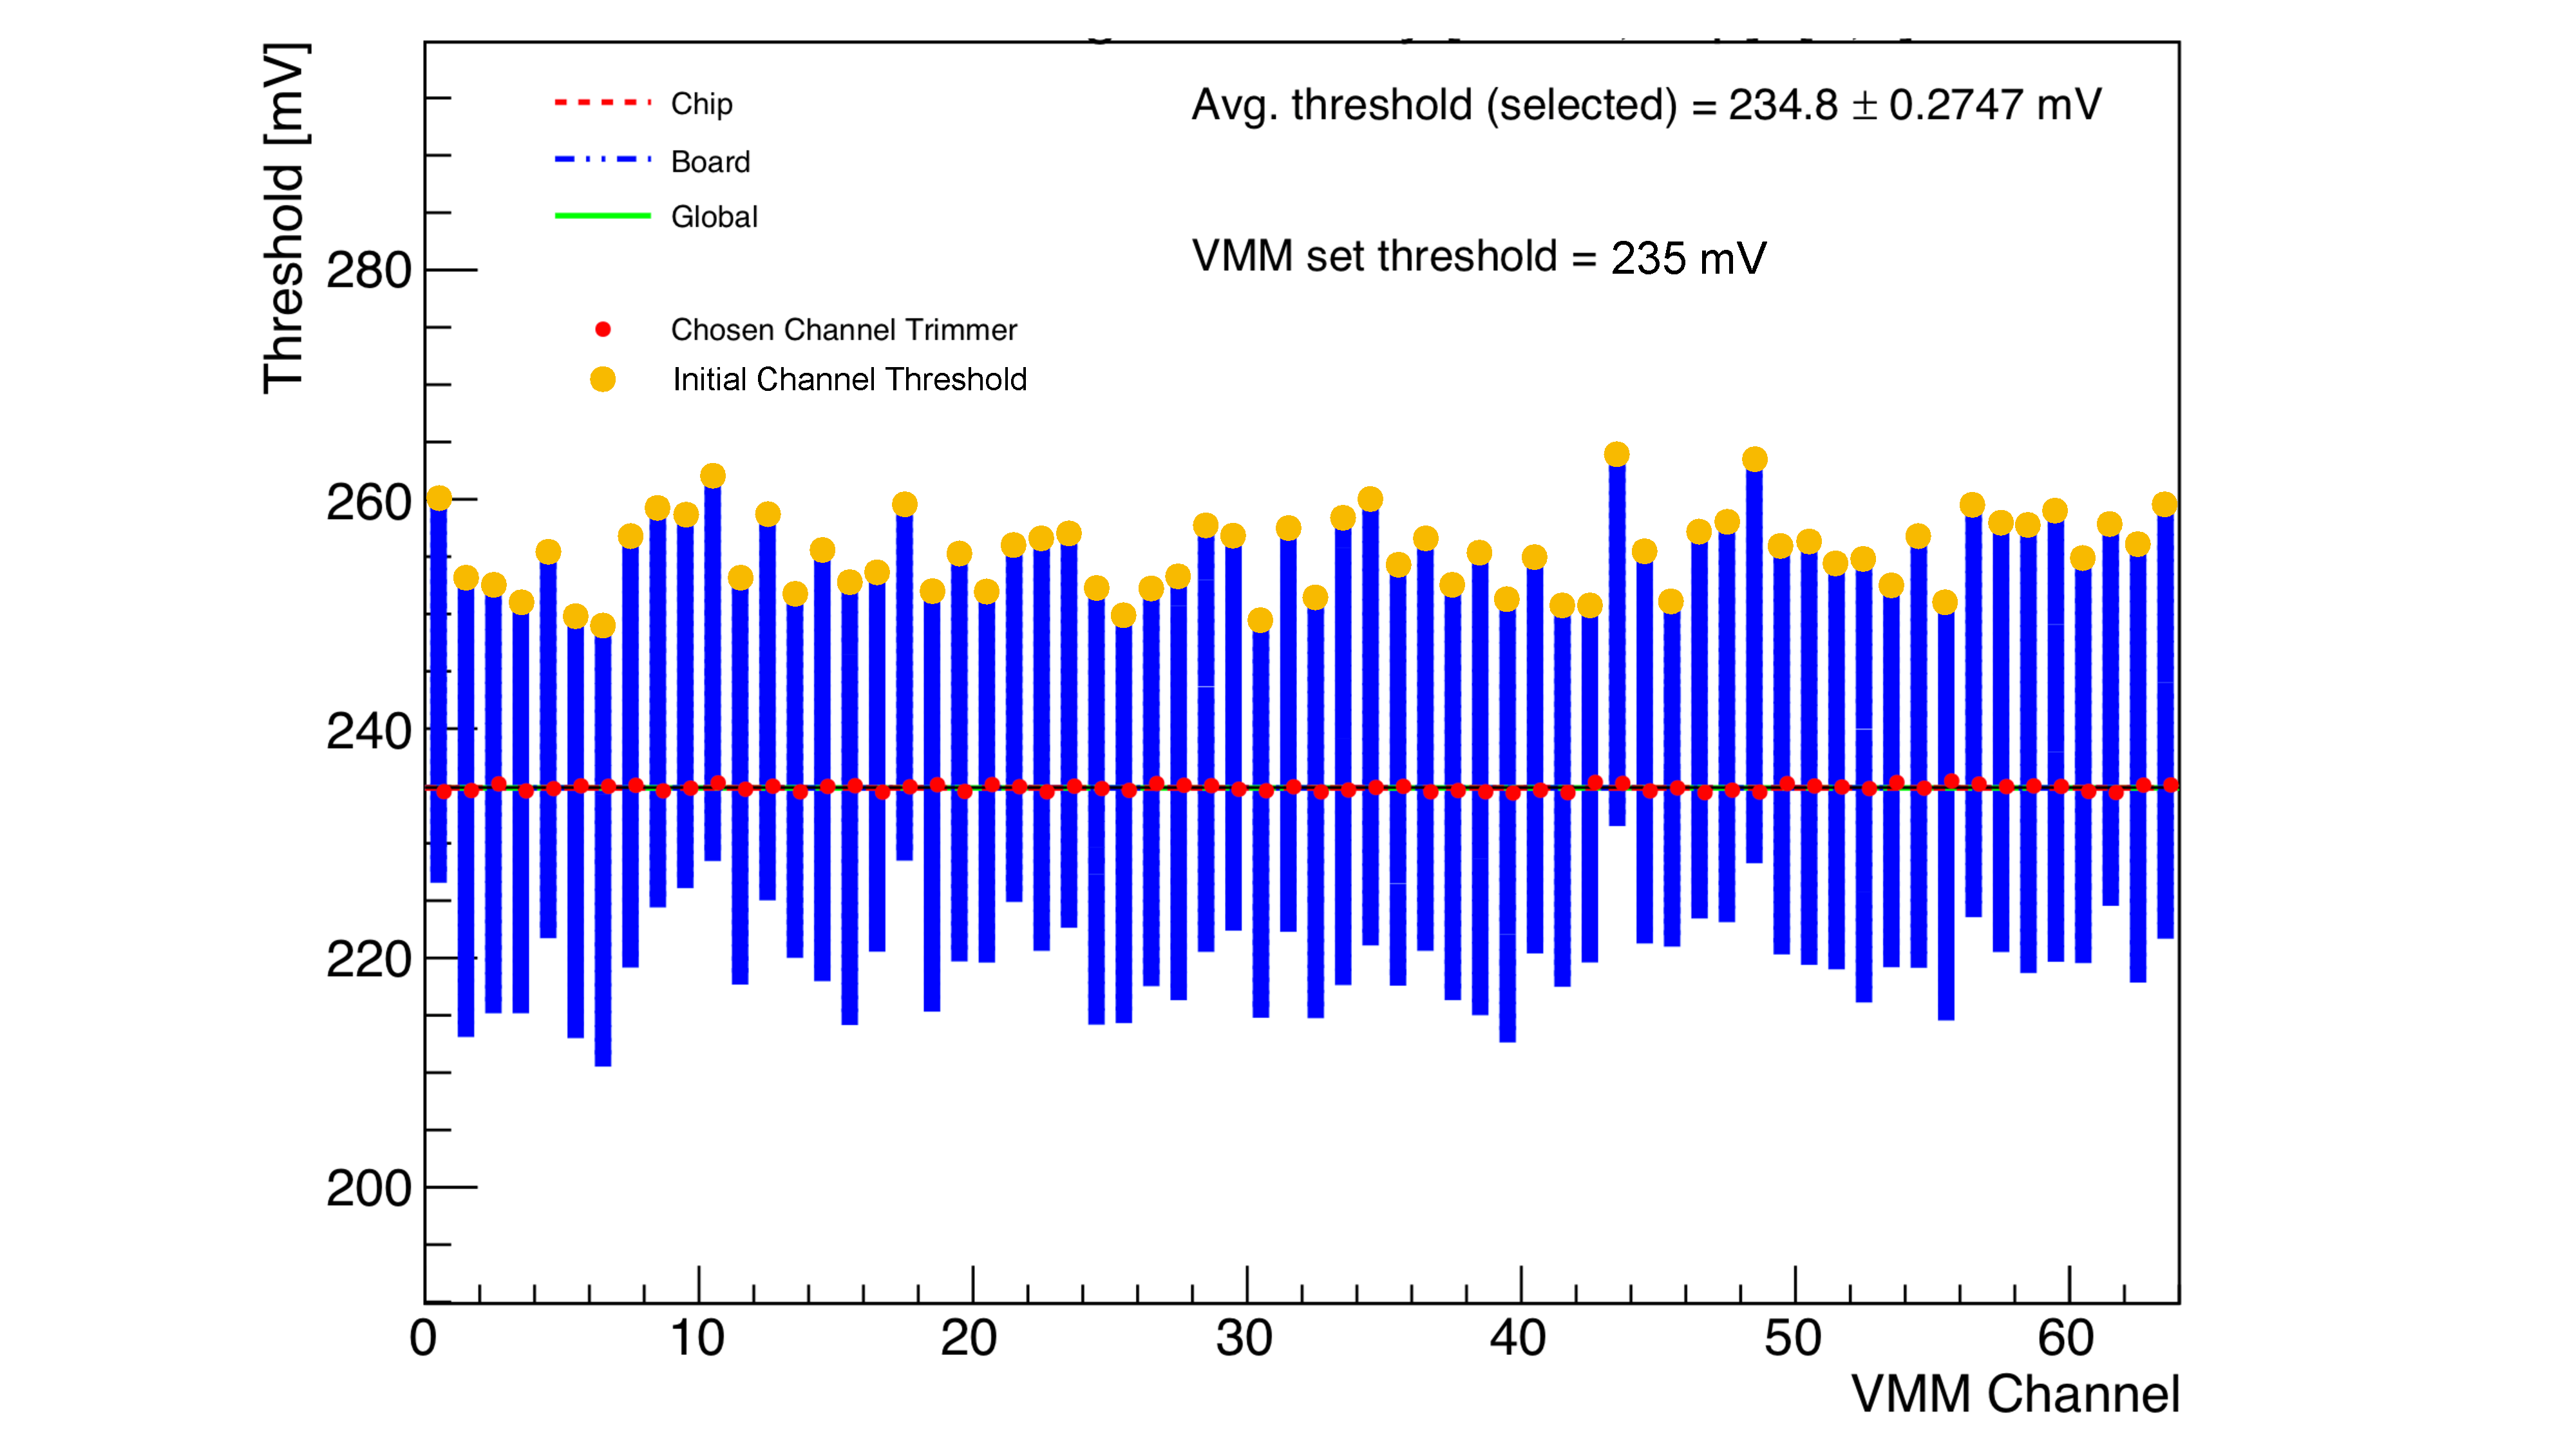
\includegraphics[width=0.85\textwidth]{figures/nsw/calibration/channel_threshold_calibPDF}
        \caption{
            Summary plot of a VMM channel threshold trimming calibration.
            For this set up, a single VMM is calibrated and has a global threshold
            set to 235\,mV using the threshold DAC.
            The channel-by-channel variation of the threshold is seen by the yellow dots,
            which indicate the per-channel threshold measurement made by the xADC prior to any
            threshold trimming.
            The blue columns indicate the entire threshold range accessible by each channel
            by scanning the full range of channel trimmers and taking xADC measurements at each.
            It can be seen that most channels have a full range of approximately 32\,mV.
            The calibration algorithm shown here picks for all VMM channels the amount of trimming
            that allows for them to have thresholds as near as possible to the globally set threshold.
            In this case, the post-calibration threshold of all channels, indicated by the red dots,
            is very nearly 235\,mV, and is $234.8\pm 0.27$\,mV on average.
        }
        \label{fig:calib_channel_trim}
    \end{center}
\end{figure}

\subsubsection{Signal Amplitude Gain and Pedestal}
\label{sec:calib_pdo}

The output of the PDO for each channel must also be calibrated.
The PDO calibration aims to correct the per-channel response to a given input
signal.
Its calibration relies on the injection of test pulses on each channel.
Measurements of the output PDO for each channel can be taken as a function
of the amplitude of the test pulse, which is configured via the 10-bit test pulse DAC.
This is illustrated on the left side of Figure~\ref{fig:gain_curves}.
Linear fits to the resulting measurements provide a measure of the channel gain, which
will generally differ with respect to the globally set VMM channel gain.
The right side of Figure~\ref{fig:gain_curves} shows the channel-by-channel slope (gain)
variation measured for a single VMM.
From the DAC-mV relation derived from the DAC calibration described above, the
observed slope can be obtained in absolute terms (i.e. in terms of mV/fC) to give the channel gain.
This can then be used
to correct the signal amplitude measurements in later analysis; for example, when constructing particle tracks.
From the measurements above, relying on the linear fits, the PDO pedestal can be measured
as the extrapolated $y$-intercept.
Due to the VMM's internal ADC having a built-in baseline subtraction, the PDO pedestal will
differ with respect to the baseline as described Section~\ref{sec:calib_baselines}.
The PDO pedestal is an offset that must be subtracted from the PDO amplitude measurements
prior to any analysis or track fitting.
The VMM can be configured to output PDO measurements for those channels that are neighboring
a channel that has an above-threshold signal but that do not themselves have an above-threshold
signal.
With this option enabled, individual channels may have injected test-pulses and have the  neighboring
channels' PDO measurements recorded.
The neighboring channels readout in this manner thus provide
an alternative method for measuring the PDO pedestal.
The neighbor-enabled method for obtaining VMM channel PDO pedestals is actually more efficient
as a significantly smaller amount of data samples need to be recorded since one does not
need to scan over values of the test pulse amplitude: pedestals obtained in this manner
can be obtained for any single value of the test pulse amplitude since they are obtained from those channels
\textit{not} being pulsed.
Figure~\ref{fig:pedestals} shows the PDO pedestals measured for the channels of a single VMM
using the linear-fit extrapolation and neighbor-enabled methods.
The two methods agree quite well with one another.

\begin{figure}[!htb]
    \begin{center}
        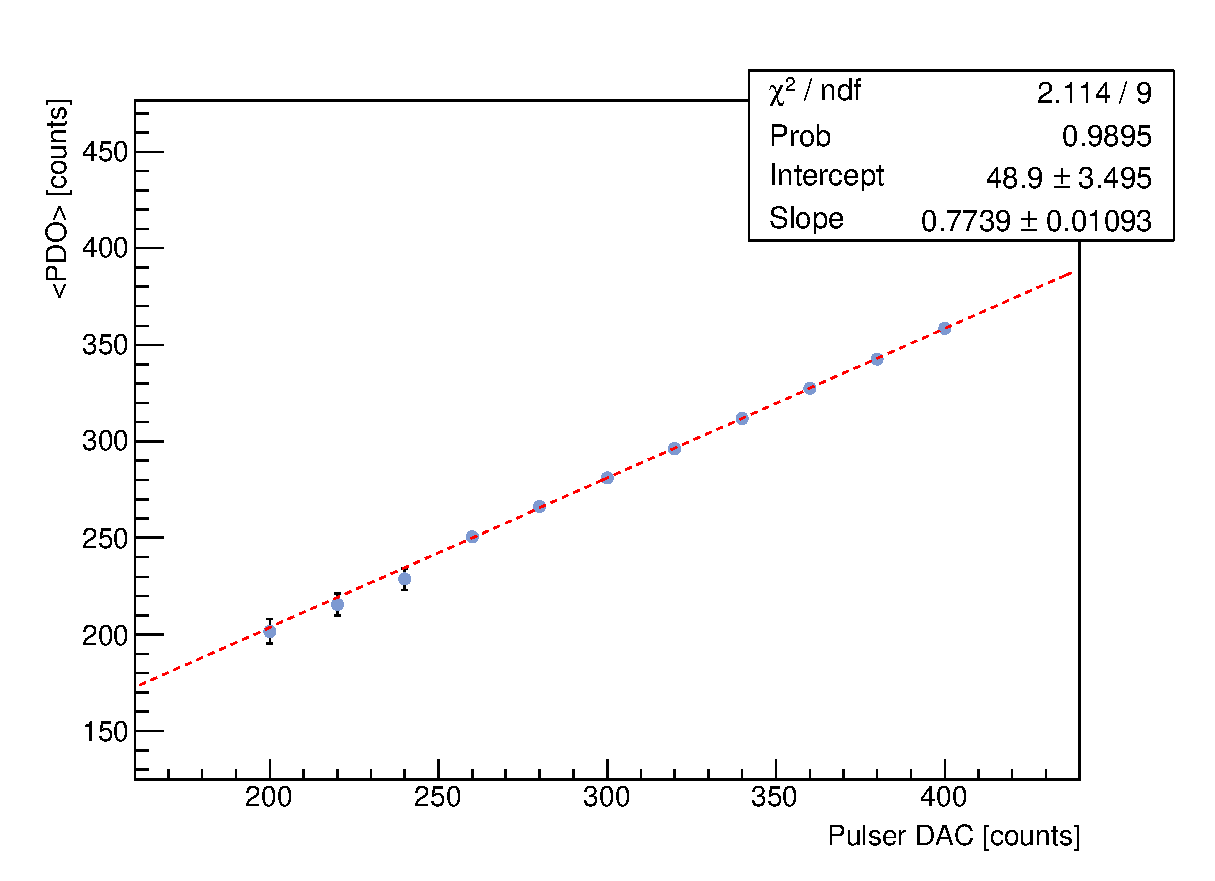
\includegraphics[width=0.5\textwidth]{figures/nsw/calibration/calib_gain_curve}
        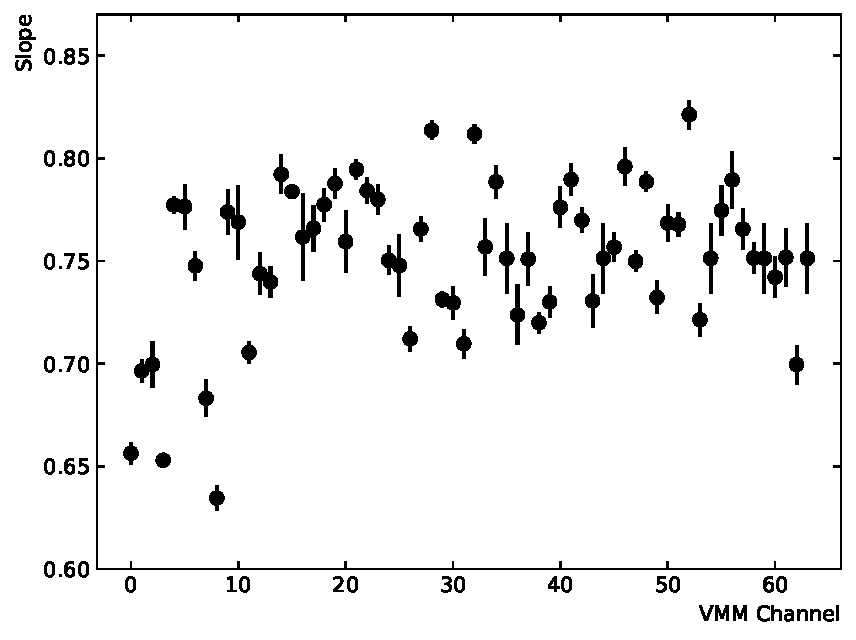
\includegraphics[width=0.45\textwidth]{figures/nsw/calibration/gain_curve_slope}
        \caption{
            \textbf{\textit{Left}}: Average PDO response as a function of test pulse amplitude,
                for a single VMM channel.
                The slope gives a measure of the channel gain.
            \textbf{\textit{Right}}: Measured slopes of the PDO response to injected test pulses
                for 64 channels of a VMM.
        }
        \label{fig:gain_curves}
    \end{center}
\end{figure}

\begin{figure}[!htb]
    \begin{center}
        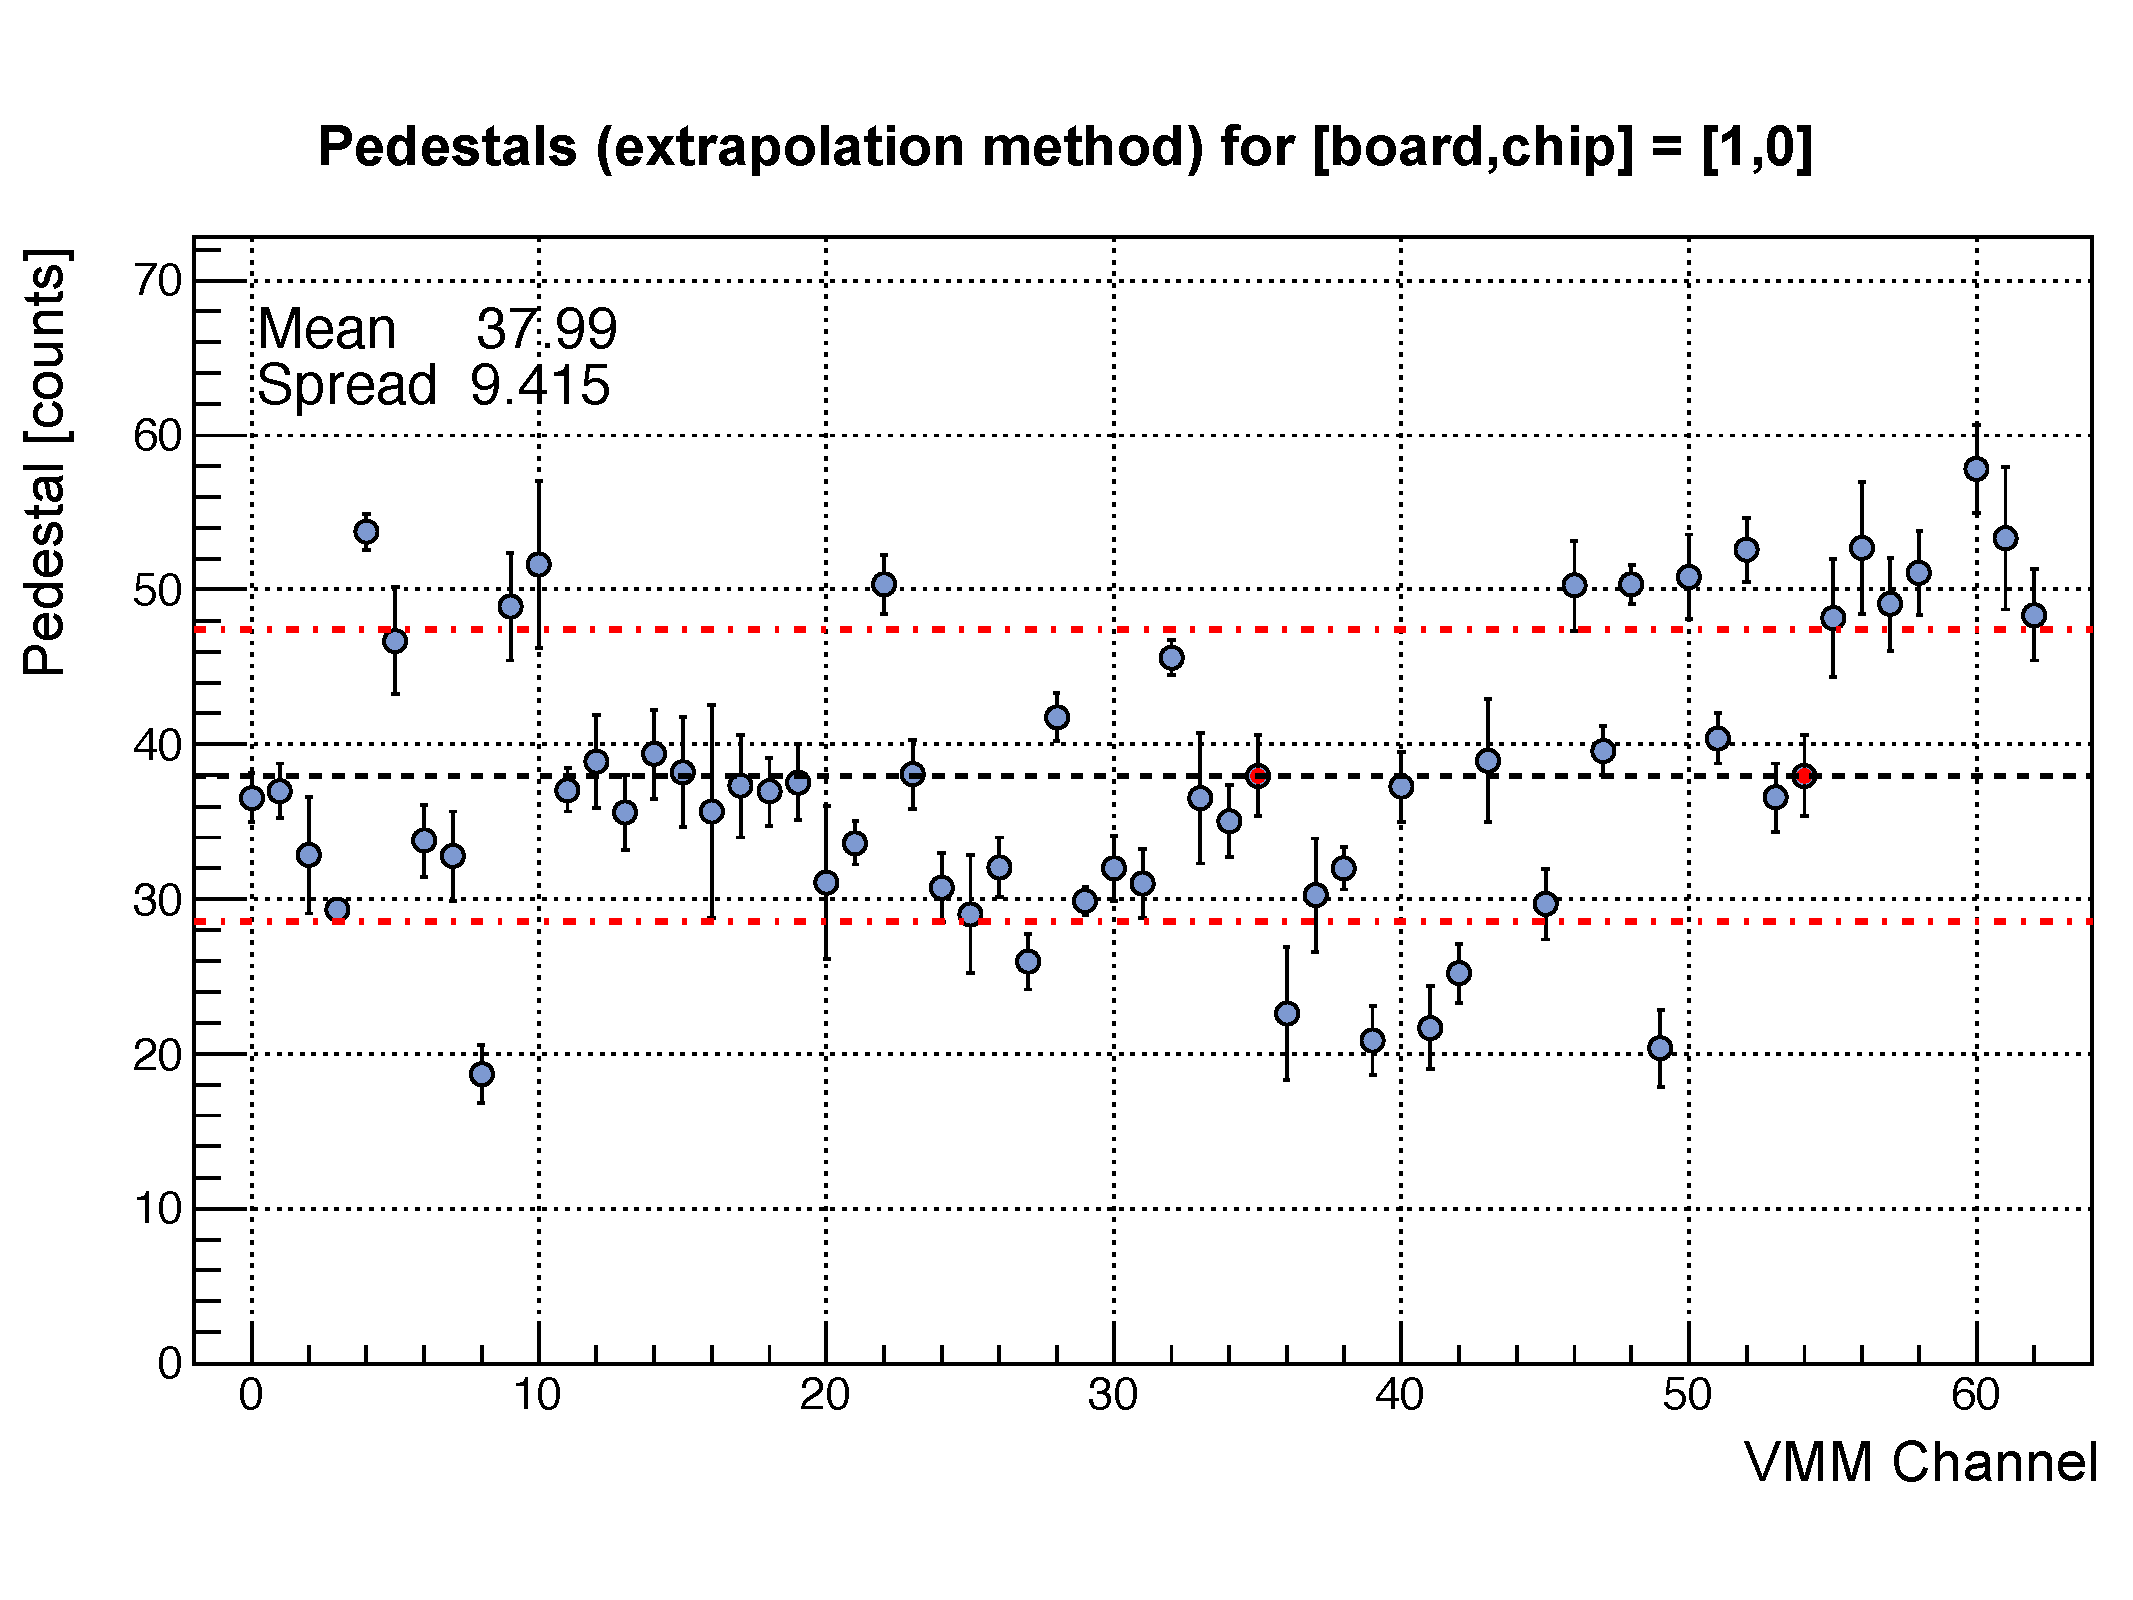
\includegraphics[width=0.48\textwidth]{figures/nsw/calibration/vmm_pedestals_extrap}
        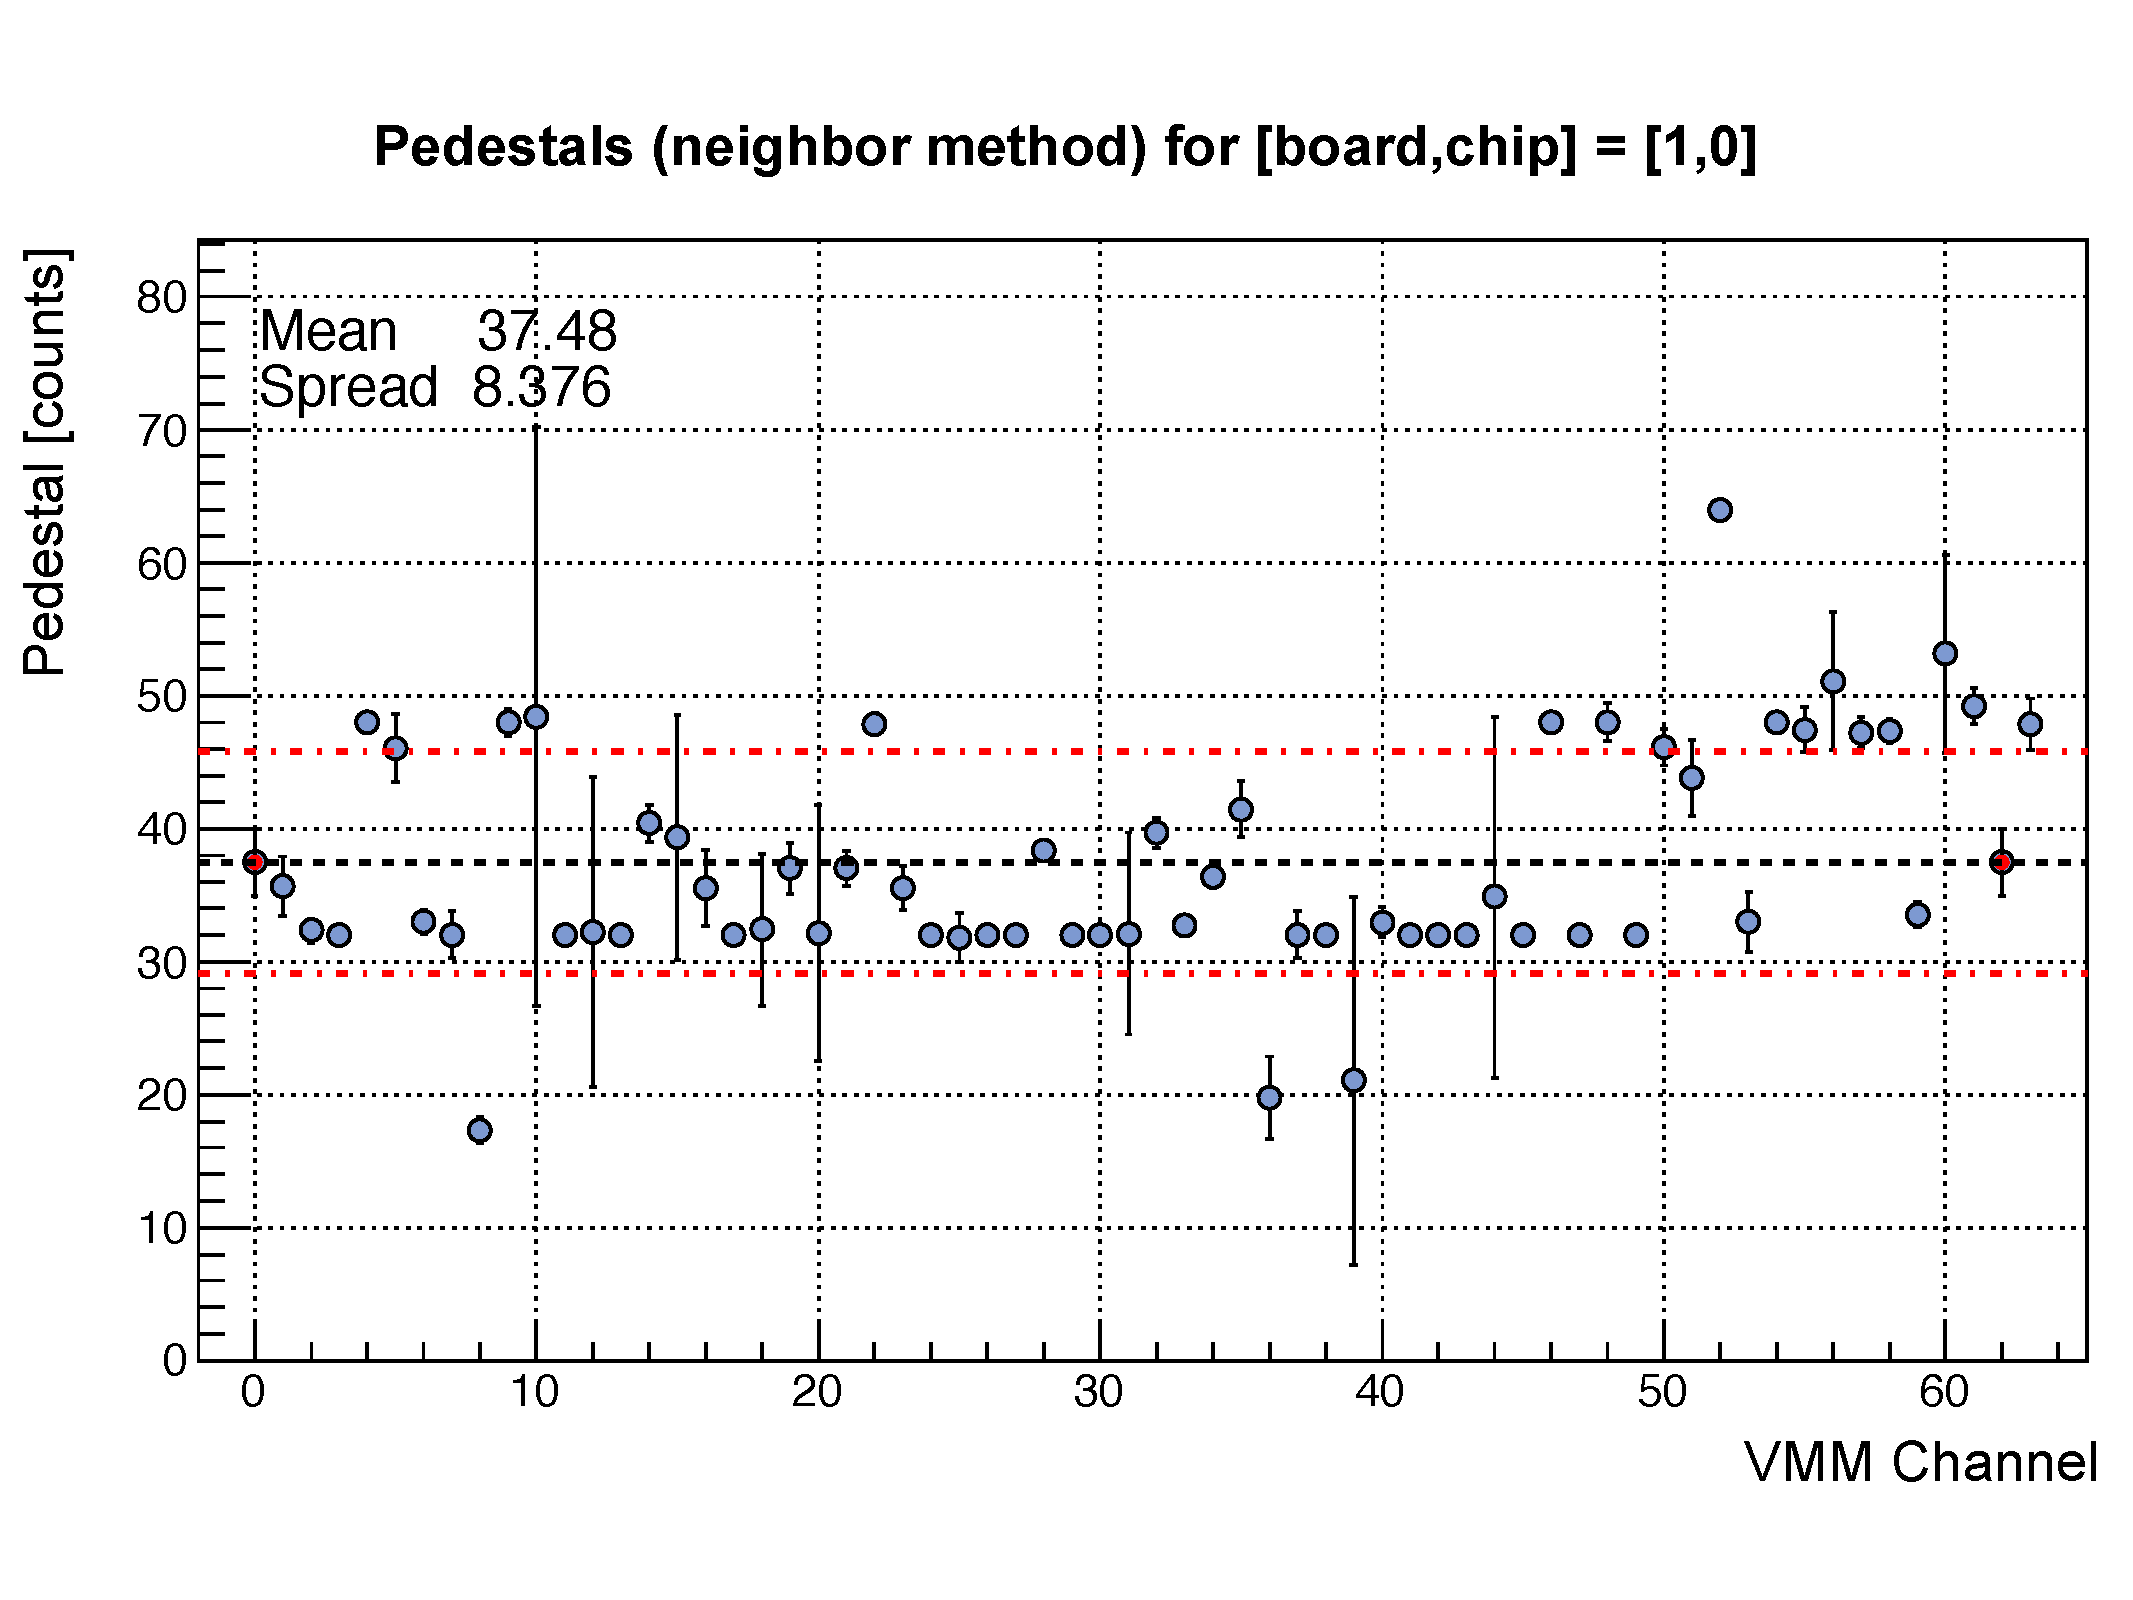
\includegraphics[width=0.48\textwidth]{figures/nsw/calibration/vmm_pedestals_neighbor}
        \caption{
            Measurements of PDO pedestals of each channel of a VMM.
            \textbf{\textit{Left}}: Using the linear-fit extrapolation method.
                The mean pedestal measured across all channels is $37.99$, in units of PDO counts.
            \textbf{\textit{Right}}: Using the neighbor method.
                The mean pedestal measured across all channels is $37.48$, in units of PDO counts.
        }
        \label{fig:pedestals}
    \end{center}
\end{figure}

\subsubsection{Timing Measurement Calibration}
\label{sec:calib_tod}

The time measurement of the MM readout is of the utmost importance for providing
high-resolution tracks since the track-primitive building in the MM detectors
relies primarily on the $\mu$-TPC reconstruction method, as illustrated on the right side of Figure~\ref{fig:mm_tpc_hit_loc}.
The TDO output must then be calibrated if high resolution track-primitives are to
be constructed.

The TDO provides signal timing information and is the the amplitude of a latched
time-to-analog converter (TAC) voltage ramp that is initiated either when the signal peak
amplitude is found (coinciding with the time at which the PDO value is latched)
or when the signal amplitude first crosses above threshold.
The former is referred to as `timing-at-peak' and the latter as `timing-at-threshold'.
The operation of the TAC ramp and subsequent TDO measurement is illustrated
in Figure~\ref{fig:tdo_illustration}.
The maximum TAC ramp time is configurable, and if the maximum is reached the output
TDO value will be saturated at its maximum value.
In nominal VMM operation, the TAC ramp is halted at the following falling-edge
of the bunch-crossing clock driving the VMM readout and read out as the TDO.
In an alternative configuration of the frontend electronics, the FPGA which
provides the bunch-crossing clock to the VMM can be configured such that
it halts the bunch-crossing clock for a fixed amount of time once the TAC ramp is
initiated.
After this fixed amount of time, the bunch-crossing clock is re-initiated and the first
falling edge then halts the TAC ramp.
This \textit{fixed latency} method of acquiring the TDO allows
for a fine-grained calibration of the timing measurement of the VMM.
The timing calibration is performed by scanning the bunch-crossing clock's latency (i.e.
the amount of time for which it is halted) and measuring the TDO output, per channel,
as a result of injected test pulses.
This is illustrated in Figure~\ref{fig:timing_calib_bcLatency} for two values of the
TAC ramp time: 100\,ns and 350\,ns.
Linear fits to the resulting TDO measurements as a function of this fixed latency
then give the per-channel conversion from TDO output (counts) to absolute time (e.g. nanoseconds).
The timing calibration using the nominal TDO measurement method is performed similarly. However, instead
of scanning the bunch-crossing clock latency, the time difference between the test pulse clock driving
the injection of the test pulse charge and the bunch crossing clock is scanned.
From Figure~\ref{fig:tdo_illustration} it can be seen that by skewing the test pulse injection in
this manner, for larger values of the time difference the TAC ramp time will be nearer to the
next subsequent bunch crossing clock and therefore will be halted sooner.
The resulting TDO measurements for several values of the amount of time skewing allows for the
timing calibration to be performed.

Once the TDO conversions are known, the inherent VMM timing resolutions can be studied and
further measurement improvements can be made.
Figure~\ref{fig:time_res} shows the TDO timing resolution in absolute time as a function
of the injected charge.
It can be seen that for input signals with charges $Q \approx \mathcal{O}(10)$\,fC
that sub-nanosecond timing resolutions are approached.
Given that the MM detector avalanche gains are on the order of $10^4$, this
leads to the VMM having sub-nanosecond timing resolutions for avalanches produced
from 1 to 2 drift electrons.

The timing measurement is highly sensitive to the signal shaping, as can be seen in Figure~\ref{fig:time_res}.
This is due to the fact that the shaped signal's peak and threshold-crossing becomes less pronounced for larger
shaper integration times, leading to poorer timing resolution.
The effect of the signal shaping also introduces non-negligible timewalk, as seen in Figure~\ref{fig:time_walk},
which shows the effect of timewalk for a VMM configured for timing-at-threshold.
The timewalk effects are exaggerated for timing-at-threshold since the point at which a
given signal rises above threshold is more susceptible to noise, in addition to the integration
time effects described previously.
For a given timing configuration, the measurement of the timewalk for a given signal amplitude
is used to correct the timing information provided by the the VMM TDO measurement and can thus
improve the subsequent track-primitive reconstruction.

\begin{figure}[!htb]
    \begin{center}
        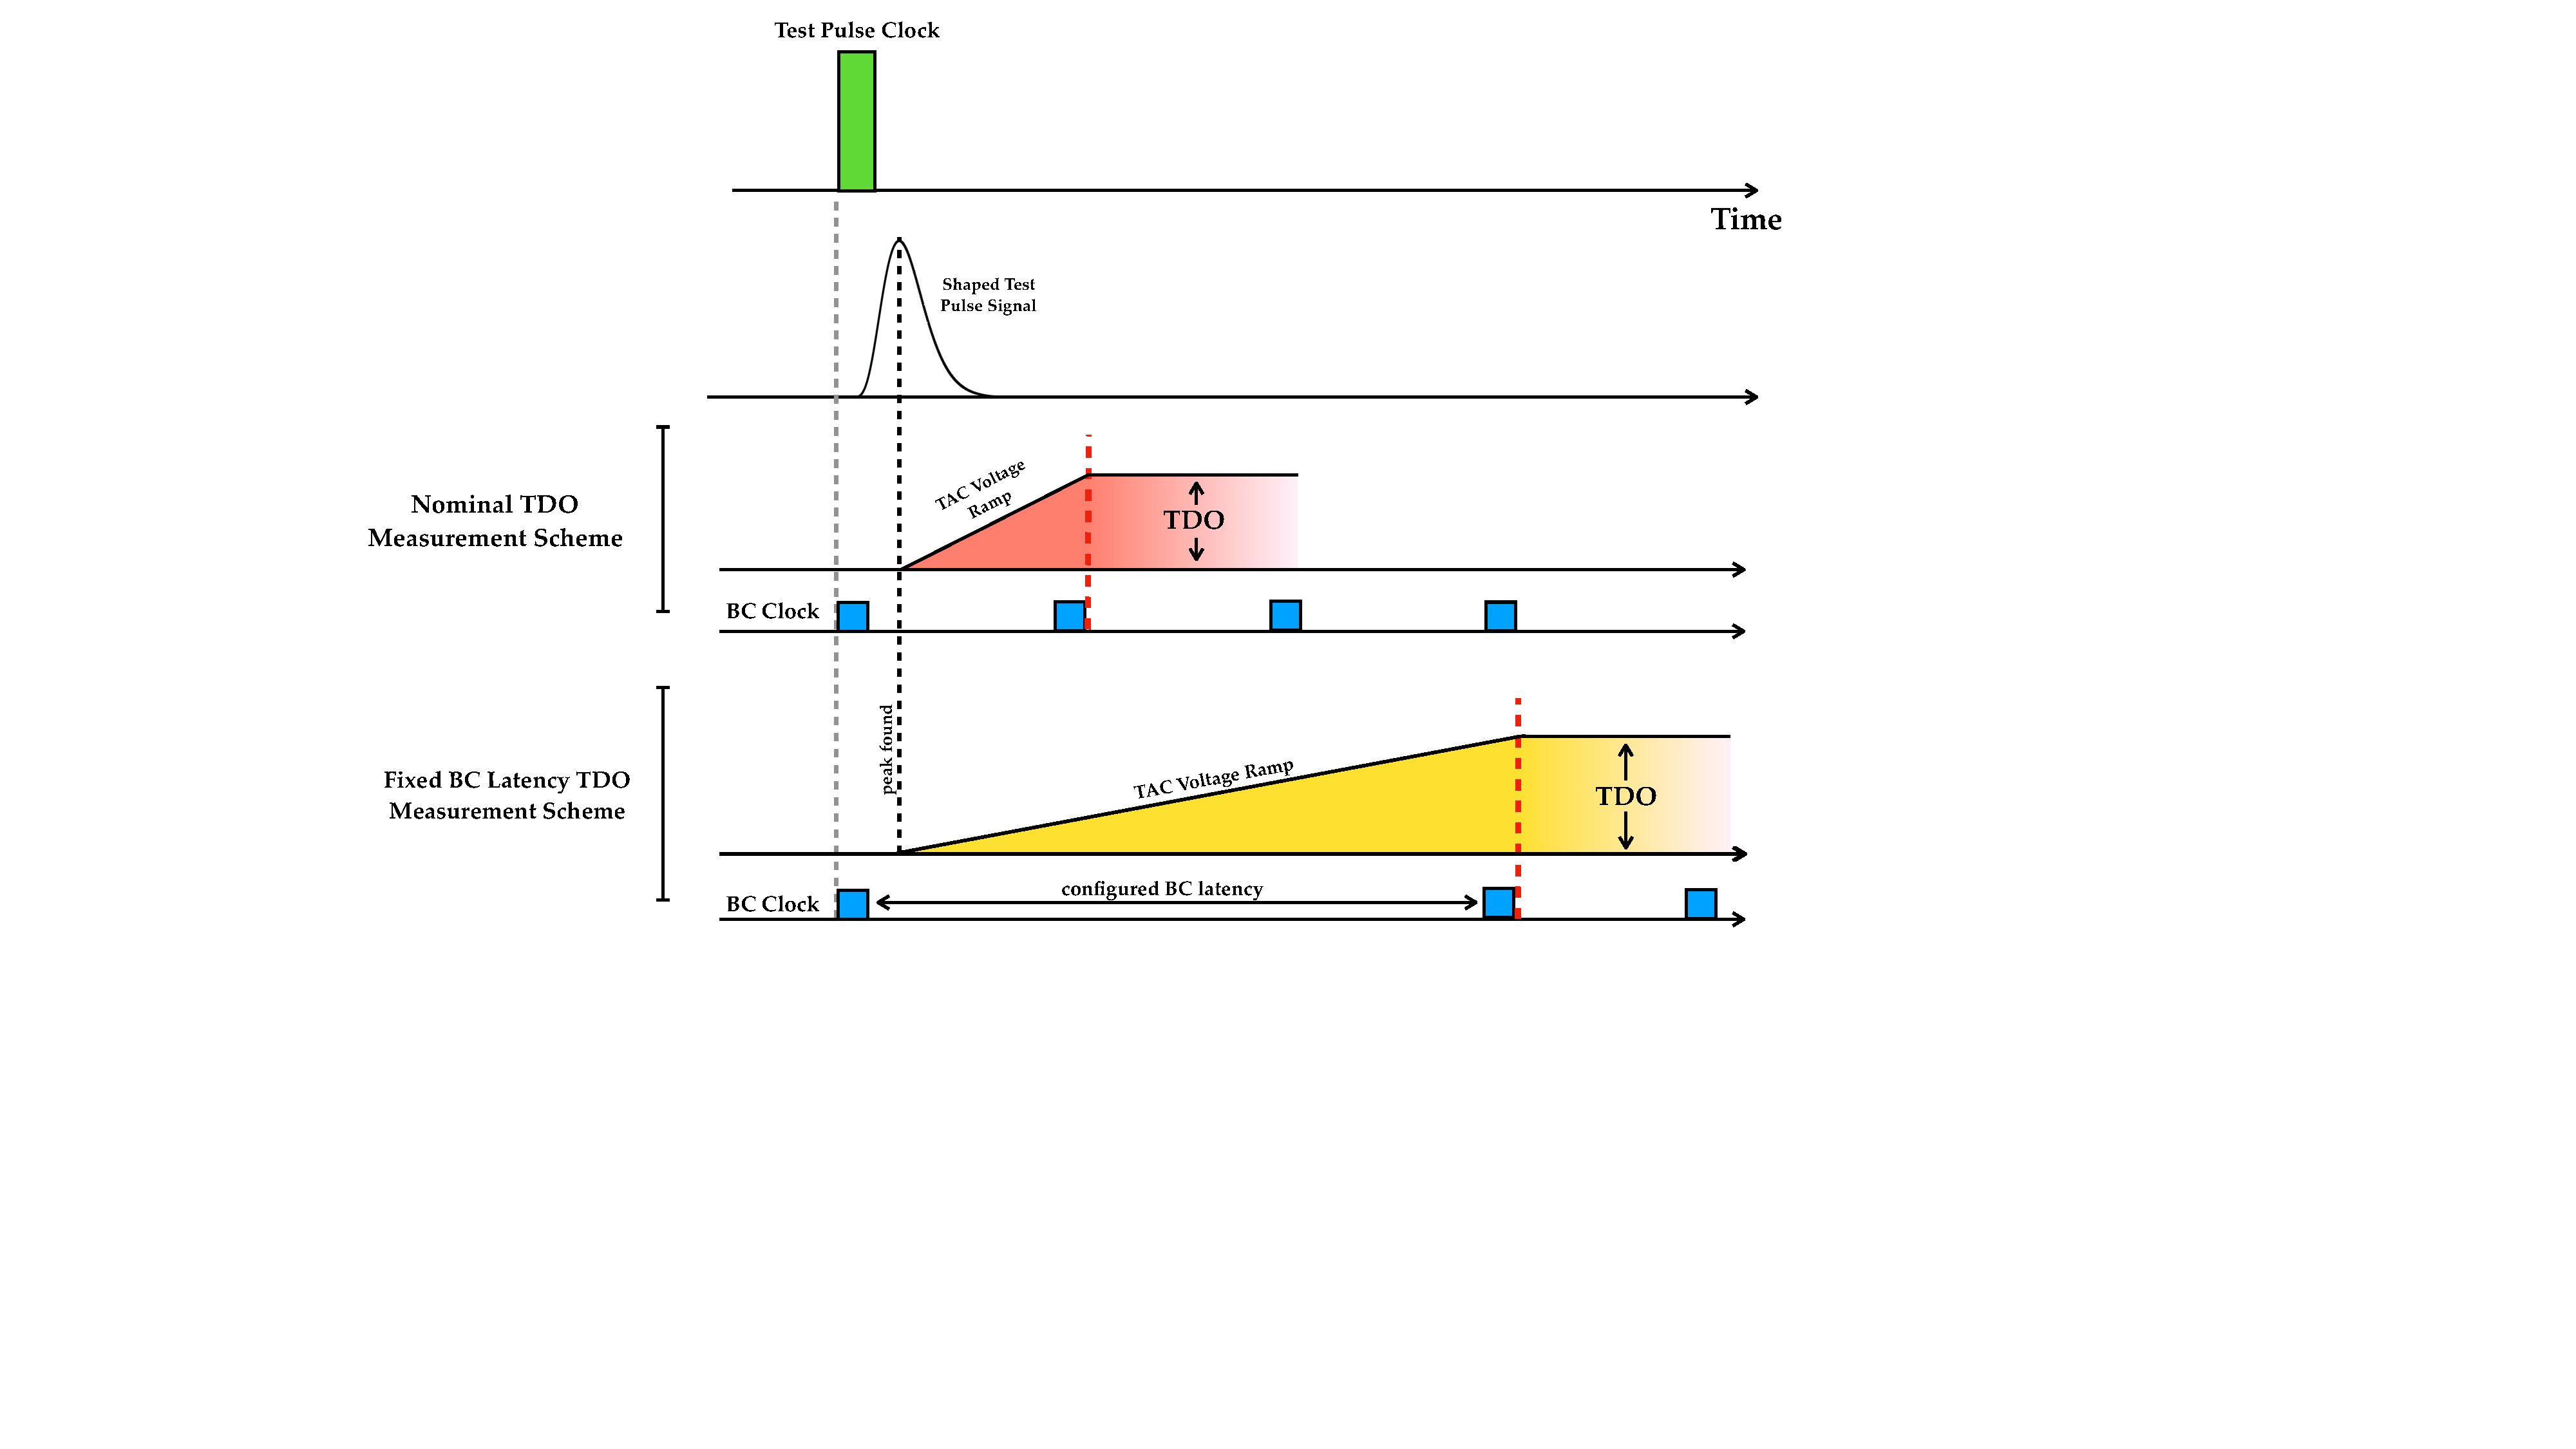
\includegraphics[width=0.8\textwidth]{figures/nsw/calibration/tdo_illustrationPDF}
        \caption{
            Illustration of the TDO measurement for an injected test pulse.
            The test pulse is injected following the test pulse clock (green), after
            which the subsequent shaped signal is formed.
            In the timing-at-peak scenario, once the peak-detector circuitry in the VMM fires,
            the TAC voltage ramp is initiated.
            In the nominal TDO measurement (red), the bunch crossing clock frequency remains unchanged
            and will be kept at its 40\,MHz frequency in LHC conditions.
            In this configuration, the next falling edge of the bunch crossing clock after
            the TAC voltage ramp begins halts the ramp, and the TAC voltage is digitised as
            the TDO value.
            While in this mode, the TAC ramp is confined to times smaller than that given by the bunch crossing
            clock frequency (25\,ns in the case of the LHC 40\,MHz clock).
            In the fixed latency mode of acquiring the TDO measurement (yellow), the bunch crossing clock
            is halted for a configurable amount of time after which it is resumed and its
            next falling edge halts the TAC voltage ramp.
            In the fixed latency mode, the TAC can ramp to its maximal configured value (60, 100, 350, or 650\,ns in the VMM3)
            if the configured BC latency is at least as large as this value.
            %Illustration of the TDO measurement for injected test pulses.
            %Here, the TAC ramp begins once the signal peak is found and halts at the next
            %falling edge of the bunch-crossing clock which drives the readout of the VMM.
            %CKTP is the clock driving test-pulse injection, CKBC is the bunch-crossing clock.
            %The TDO is the digitised voltage value corresponding to the latched TAC ramp.
            %In the nominal VMM operation mode, with a fixed CKBC frequency, the
            %window between the peak found and CKBC is bounded by the CKBC period (25\,ns for the 40\,MHz LHC bunch-crossing clock).
            %In the fixed-latency mode of operation described in the text, the CKBC is halted
            %for a fixed amount of time once the TAC ramp begins.
            %In this scenario, the TAC can ramp to its maximal value if the latency is set to
            %be longer than this value.
        }
        \label{fig:tdo_illustration}
    \end{center}
\end{figure}

\begin{figure}[!htb]
    \begin{center}
        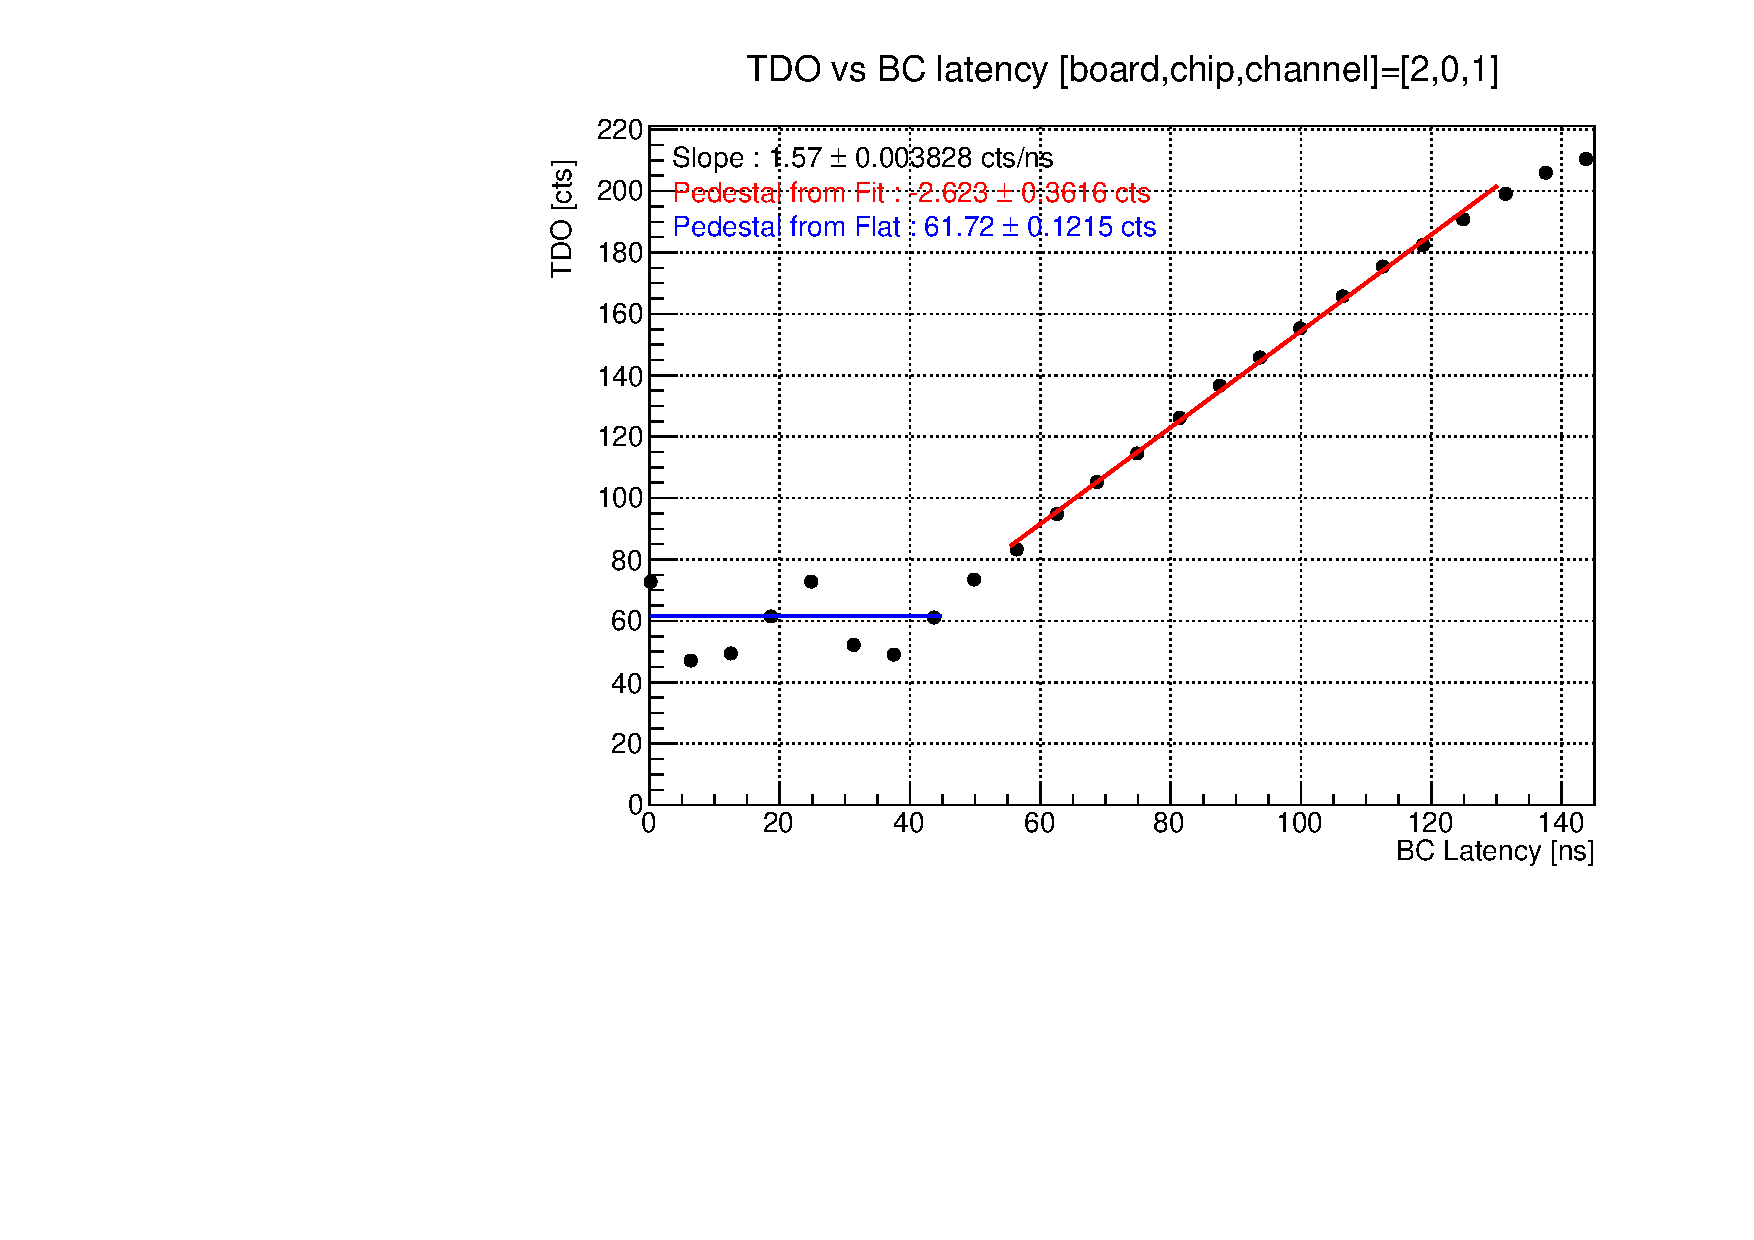
\includegraphics[width=0.48\textwidth]{figures/nsw/calibration/timing_calib_bcLatency_TAC100}
        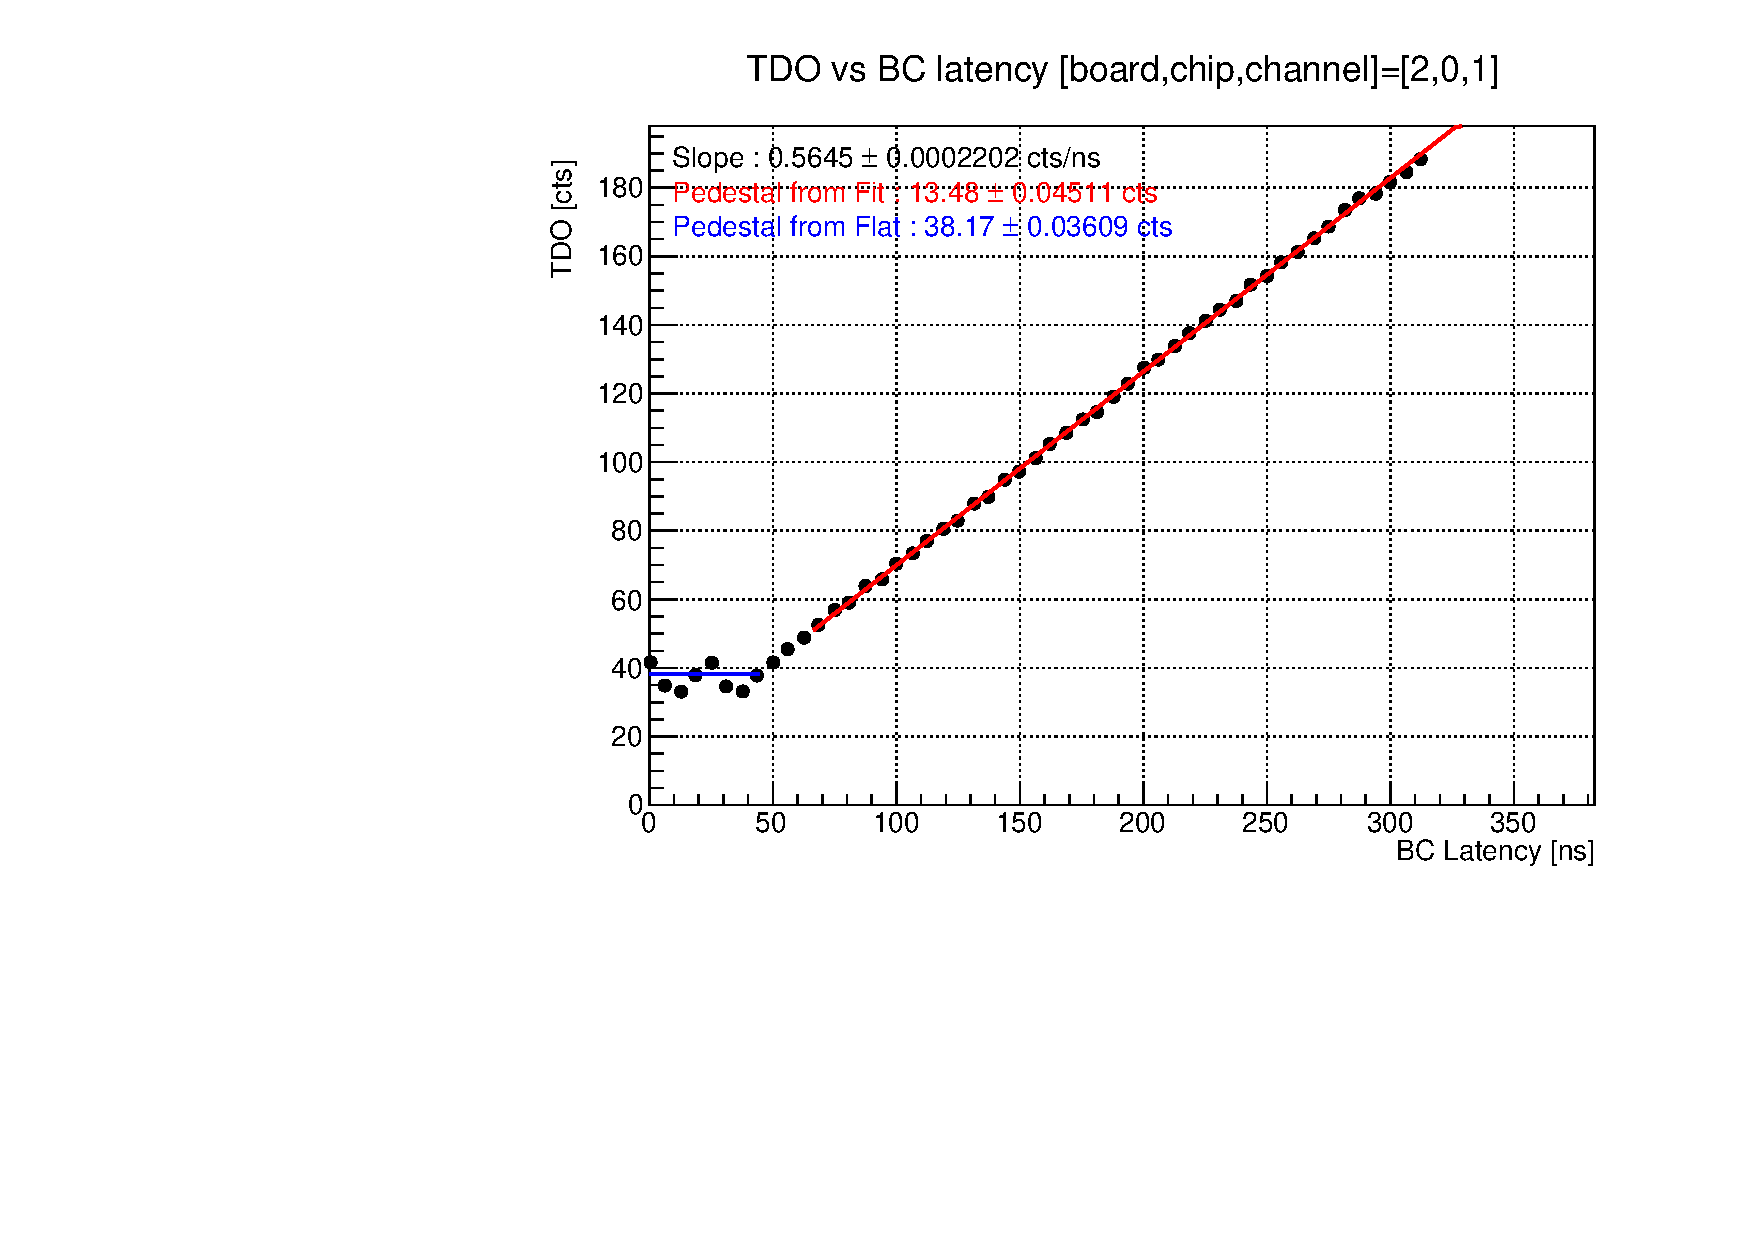
\includegraphics[width=0.48\textwidth]{figures/nsw/calibration/timing_calib_bcLatency_TAC350}
        \caption{
            TDO calibration using the fixed-latency method for a TAC ramp time of 100\,ns (\textbf{\textit{left}})
            and 350\,ns (\textbf{\textit{right}}).
            The flat portion, fit with a blue line, are 50\,ns long and correspond to the configured
            VMM shaper's integration (peaking) time.
            As can be inferred by Figure~\ref{fig:tdo_illustration}, proper timing measurements for times
            smaller than the integration time cannot be obtained.
            The linear fit for latencies beyond the peaking time give the timing calibration for the channel via
            the slope which gives the conversion between the TDO digitised count values to absolute
            time in nanoseconds.
            It can be seen that the TDO conversion constant is larger for smaller TAC ramp times,
            which follows from the fact that the TDO 8-bit range is the same irrespective of the configured
            TAC ramp.
        }
        \label{fig:timing_calib_bcLatency}
    \end{center}
\end{figure}

\begin{figure}[!htb]
    \begin{center}
        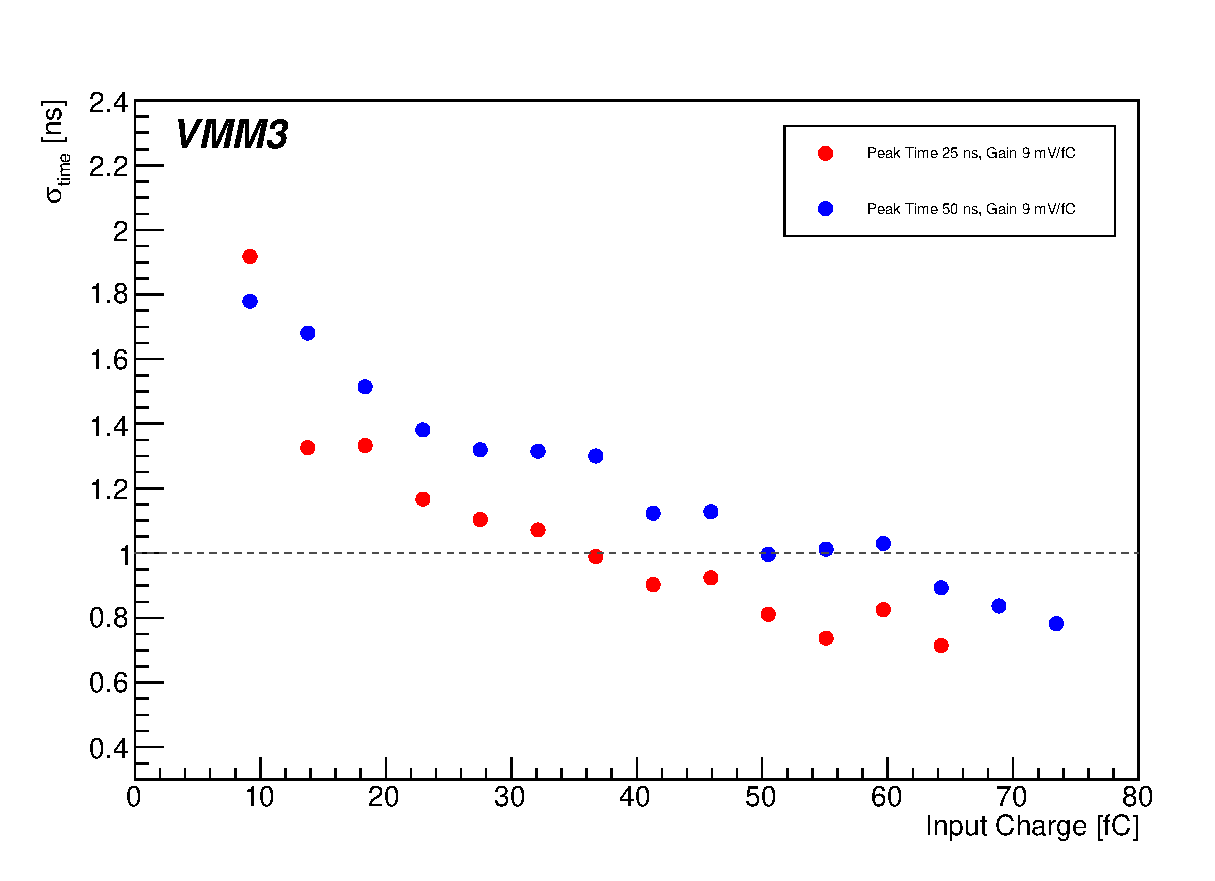
\includegraphics[width=0.48\textwidth]{figures/nsw/calibration/res_v_charge}
        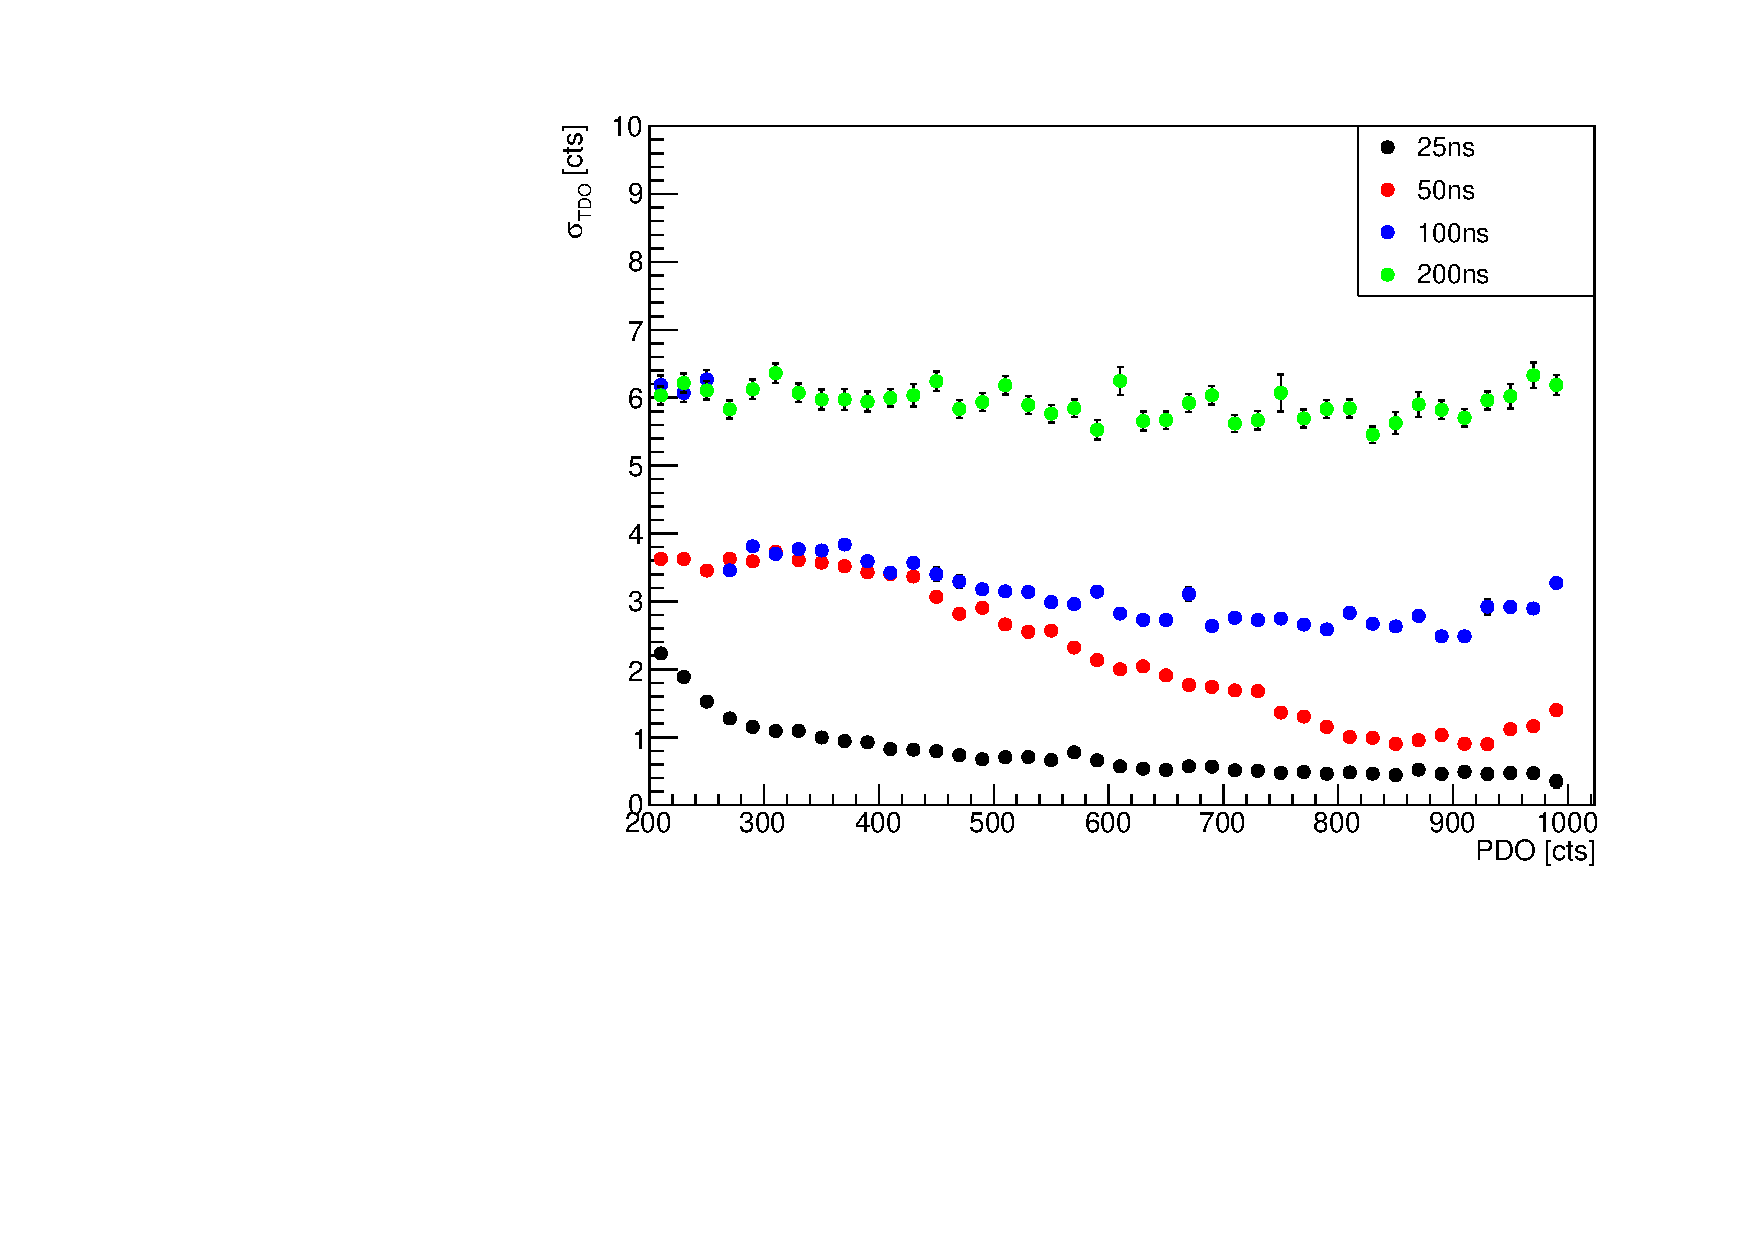
\includegraphics[width=0.48\textwidth]{figures/nsw/calibration/nsw_time_res}
        \caption{
            VMM timing resolution as a function of the injected test pulse charge
            for various integration times.
            \textbf{\textit{Left}}: Absolute timing resolution as a function of absolute charge
                for shaper integration times of 25\,ns (red) and 50\,ns (blue).
            \textbf{\textit{Right}}: TDO resolution as function of injected test-pulse
                amplitudes, over the full PDO range, for various shaper integration times: 25\,ns (black), 50\,ns (red),
                100\,ns (blue), and 200\,ns (green).
        }
        \label{fig:time_res}
    \end{center}
\end{figure}


\begin{figure}[!htb]
    \begin{center}
        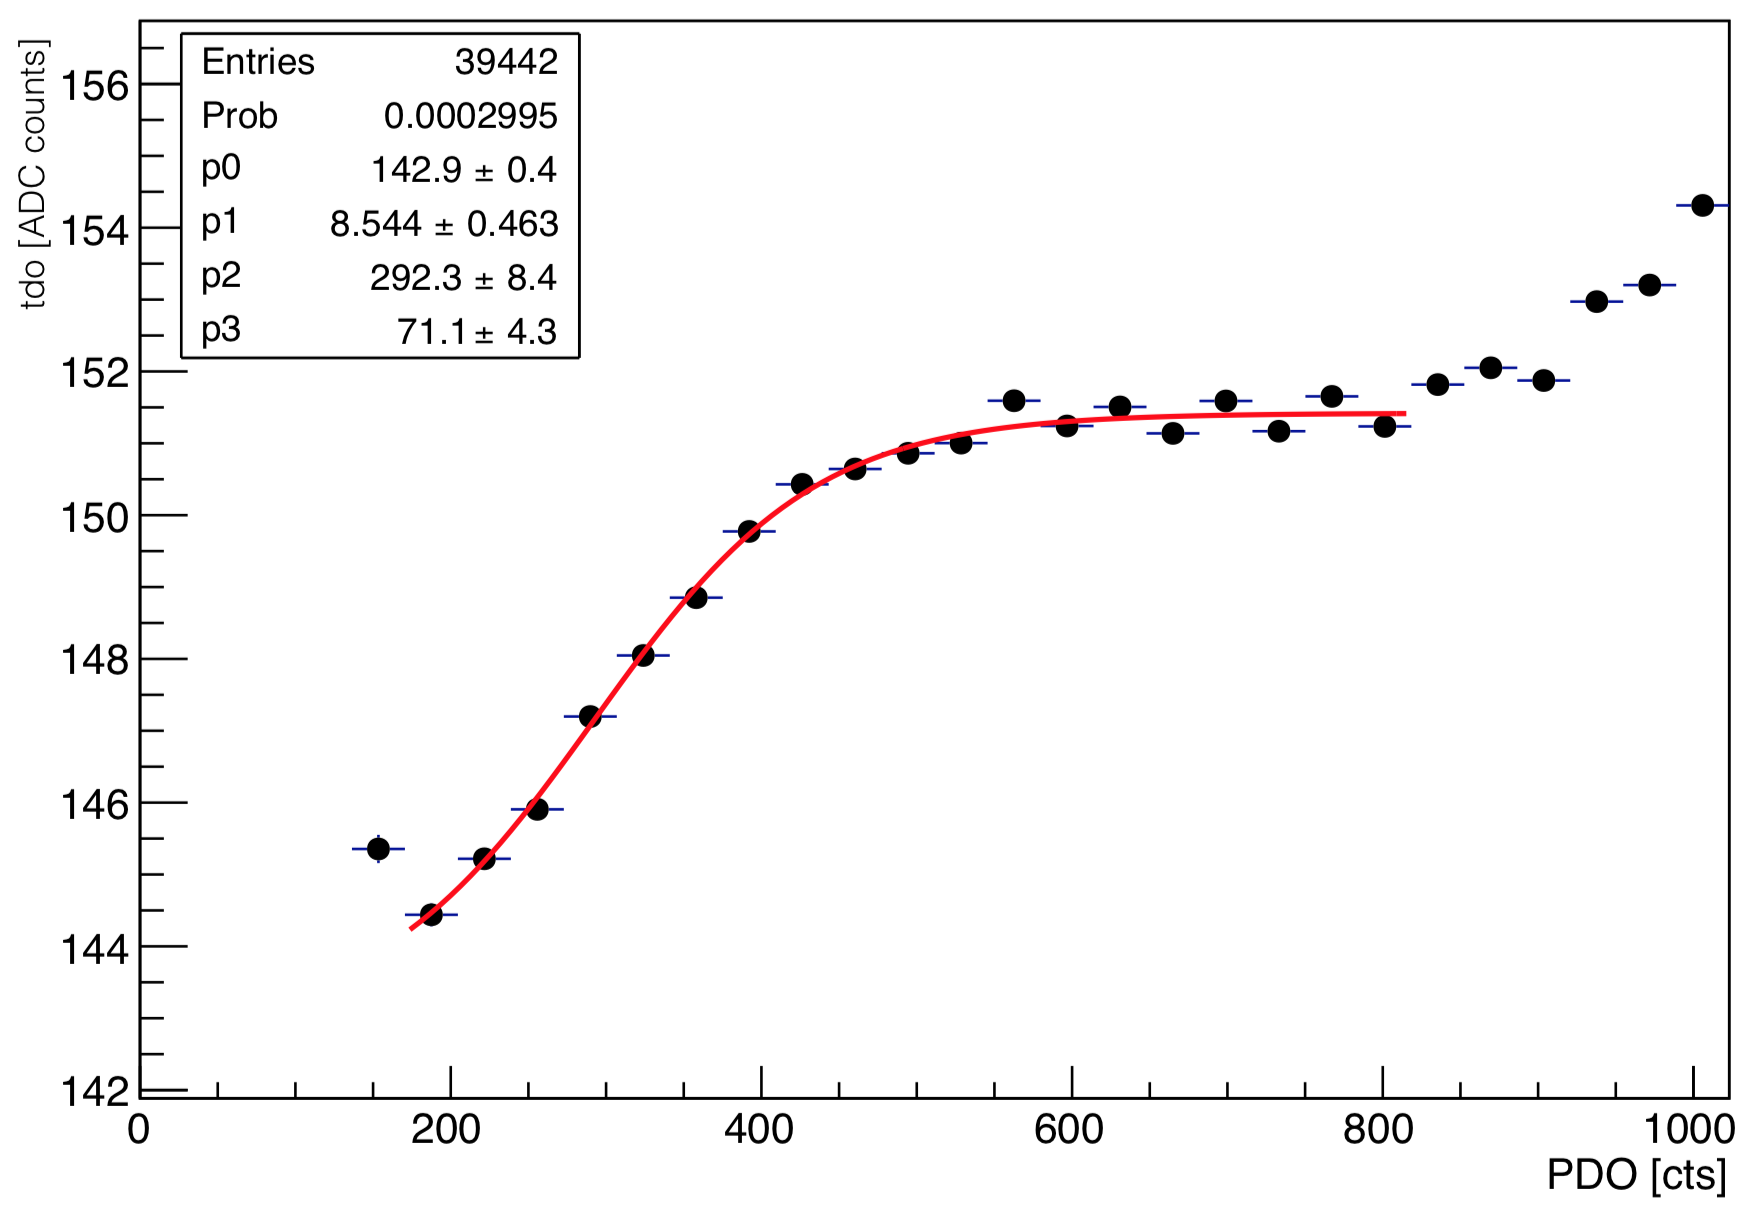
\includegraphics[width=0.48\textwidth]{figures/nsw/calibration/time_walk}
        \caption{
            Measured timewalk for a given VMM channel configured for timing-at-threshold.
            The $x$-axis is the measured PDO value of the channel and the $y$-axis is the
            TDO value, giving the time information of the signal.
            The red line is a fit to a sigmoid-like function: $\text{TDO} =  p_0 / (p_1 + p_2 * e^{p_3 \times \text{PDO}})$.
            The injected signals all occur at the same time, but due to the timewalk effects
            the measured time provided by the TDO measurement are biased to larger values as the measured amplitude
            increases.
        }
        \label{fig:time_walk}
    \end{center}
\end{figure}

